\documentclass[12pt]{article}
\usepackage[a4paper,
	left=1in,
	right=1in,
	top=1in,
	bottom=1in]{geometry}
\usepackage{tikz}
\usetikzlibrary{positioning,arrows}
\usetikzlibrary{decorations.pathmorphing}
\usetikzlibrary{decorations.markings}
\usepackage{gensymb}
\usepackage{amsmath}
\usepackage{cancel}
\usepackage{xcolor}
\usepackage{amssymb}
\usepackage{graphicx}
\usepackage{systeme}
\usepackage{hyperref}
\usepackage{pgfplotstable,filecontents}
\pgfplotsset{compat=1.9}
\usepackage{listings}
\usepackage{subcaption}
\usepackage{setspace}
\usepackage{relsize}
\usepackage{bigints}
\usepackage{lscape}
\usepackage{caption}
\usepackage{neuralnetwork}
\usepackage{indentfirst}
\usepackage{amsmath}
\usepackage{sectsty}
\usepackage{textcomp}
\usepackage{gensymb}
\usepackage{mathtools, cuted}
\usepackage{subcaption}
\usepackage{csquotes}
\usepackage{setspace}
\usepackage{times}
\usepackage[scaled=0.9]{DejaVuSansMono}

\renewcommand\arraystretch{1.5}
\renewcommand{\thefootnote}{\fnsymbol{footnote}}
\sectionfont{\fontsize{12}{15}\selectfont}
\subsectionfont{\fontsize{12}{15}\selectfont}
\subsubsectionfont{\fontsize{12}{15}\selectfont}


\definecolor{codegreen}{rgb}{0,0.6,0}
\definecolor{codegray}{rgb}{0.5,0.5,0.5}
\definecolor{codepurple}{rgb}{0.58,0,0.82}
\definecolor{backcolour}{rgb}{0.95,0.95,0.92}


\lstdefinestyle{mystyle}{
	backgroundcolor=\color{backcolour},   
	commentstyle=\color{codegreen},
	keywordstyle=\color{magenta},
	numberstyle=\tiny\color{codegray},
	stringstyle=\color{codepurple},
	basicstyle=\ttfamily\scriptsize,
	breakatwhitespace=false,         
	breaklines=true,                 
	captionpos=b,                    
	keepspaces=true,                 
	numbers=left,                    
	numbersep=5pt,                  
	showspaces=false,                
	showstringspaces=false,
	showtabs=false,                  
	tabsize=4
}
\lstset{style=mystyle}

\setlength\parindent{24pt}

\tikzset{
	particle/.style={thick,draw=black, postaction={decorate},
		decoration={markings,mark=at position .5 with {\arrow[black]{triangle 45}}}},
	gluon/.style={decorate, draw=black,
		decoration={coil,aspect=0}}
}


\tikzset{%
	every neuron/.style={
		circle,
		draw,
		minimum size=1cm
	},
	neuron missing/.style={
		draw=none, 
		scale=4,
		text height=0.333cm,
		execute at begin node=\color{black}$\vdots$
	},
}

\newcommand{\etl}{\textit{et al.}}
\sloppy


\begin{document}
\section*{ABSTRACT\centering}

Security and privacy is one of most basic human rights, that should be provided, regardless of the significance of human life. However, due to inefficiency of traditional methods currently in use, security and privacy rights can easily be bypassed and voided. Thus the study aims to implement a robust and secure system that will protect the security and privacy rights. 

The researchers utilized RFID technology and Arduino board, and machine learning models of face recognition, which was evaluated for use as lock access, attendance checking, and security system. A complementary regression model was also devised to assess the cost effectiveness of Arduino-based systems.

It was found that RFID and Arduino-based lock access systems have an average unlock and lock time of $\mu_{unlock} = 2.80s$, and $\mu_{lock} = 6.60s$, and is $\approx 20 \pm 2\%$ more cost efficient than traditional lock access systems, while the machine learning face recognition models can $\approx 59 \pm 1\%$ classify faces correctly, with an average speed of $\mu_{t} = 0.44s$, at a $30 \pm 20\%$ computation power.

Results showed that RFID and Arduino-based lock access systems are more efficient and robust than traditional methods, due to their hidden lock system and string comparison algorithm. And despite of the drawbacks and early stages of the model, it has an above average performance. Thus it is concluded that RFID and Arduino, and machine learning models of face recognition, are suitable as replacement for traditional lock, attendance checking, and security system, respectively.

\emph{\textbf{Keywords:} artificial intelligence, arduino, security, machine learning, cutting edge technologies}

\newpage
\doublespacing
\section*{THE PROBLEM AND ITS BACKGROUND\centering}
\subsection*{Introduction\centering}

Regardless of the significance of human life as both argued as important and non-significant by anthropic principle (Weinberg, 1989; Barrow \& Tipler, 1988; Schrodinger, 1944) and the laws of nature (Kaku, 1995), respectively. Providing the rights, specifically security and privacy is arguably an utmost necessity. However, due to the inefficiency and high vulnerability of traditional systems and the technology itself, it is easily bypassed, and voided at worst. Furthermore, the exponential increase of technological advancements (Kaku, 1995) and the revolution it provides in understanding  of the grand design (Katori \etl, 2022), consequently allowed the increased acceleration of security and privacy threats, and its metamorphosis to cyberspace, such examples are telemetry, spywares and ransomwares. Hence efforts are made to yield products that would prevent and decrease the progression of threat.

One of the yields from continuous efforts against security and privacy violation and exploitation in cyberspace is the movement towards free and open source software (FOSS), while increased and improved locking mechanism has been the direction of combat against physical threats, and combination of both has also shown to be effective. Nevertheless, both measures have its own advantages and disadvantages, such as FOSS softwares have an exposed vulnerabilities the attacker and public user can exploit or patch, and allows to be modified for certain needs, due to the accessible code base and algorithms. Physical measures on the other hand ascertain the decreased vulnerability of the mechanism, however with high expense and intensive maintenance.

Due to the accelerating improvement of technologies, it is necessary to keep up with the changes. Since stabilization is not sufficient, implementation is necessary as everyone is affected by changes in macro and micro level due to the interconnectivity (Lewin \etl, 2018; Lewin \etl, 2022) of organisms, thus a successful implementation of technological advancements would yield a benefit to the particular society. Hence, the goal of the study is to implement the cutting edge technological advancements, specifically RFID and Arduino, and machine learning models of face recognition.

\subsection*{Review of Related Literature\centering}

This section presents the review of related literature and studies regarding the mechanisms and theoretical principle of RFID, electromagnetism, algorithms and the programming languages, and the derivation of the equations presented in the later section.

According to Standard Model of Quantum Physics (Giancoli, 2016) the electromagnetic waves are carried by specific quanta, photons, $\gamma$, that are product of electron-electron ($e^{-}$) interactions as shown by Feynman diagram:
	
	\begin{figure}[h]
		\begin{center}
			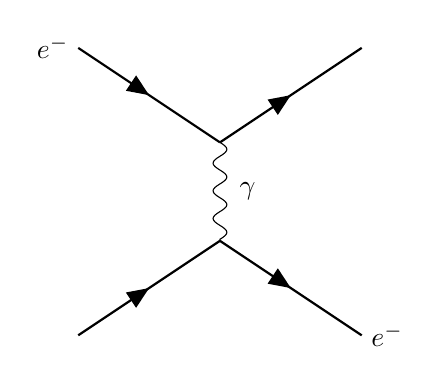
\begin{tikzpicture}[node distance=1.2cm and 1.8cm] \centering
				\coordinate[label=left:$e^{-}$] (e1);
				\coordinate[below right=of e1] (aux1);
				\coordinate[above right=of aux1] (e2);
				\coordinate[below=1.25cm of aux1] (aux2);
				\coordinate[below left=of aux2] (e3);
				\coordinate[below right=of aux2,label=right:$e^{-}$] (e4);
				
				\draw[particle] (e1) -- (aux1);
				\draw[particle] (aux1) -- (e2);
				\draw[particle] (e3) -- (aux2);
				\draw[particle] (aux2) -- (e4);
				\draw[gluon] (aux1) -- node[label=right:$\gamma$] {} (aux2);
			\end{tikzpicture}
		\end{center}
		\caption{Electron-electron interaction as shown by Feynman's diagram.}	
		\label{fig:1}
	\end{figure}
	
Where as the wave function, $\phi(\{\boldsymbol{r_i \sigma_i}\})$, and its energy, $E^{e}_{v}$ are given by:

	\begin{equation}
		H^{e} = \mathlarger{\sum_{k=1}^{N}} - \frac{\hbar}{2m} \nabla^{2}_{r_{k}} + \mathlarger{\sum_{k=1}^{N}} v(\boldsymbol{r_{k}}) + \frac{1}{2} \frac{1}{4\pi \epsilon_{0}} \mathlarger{\sum_{\substack{k, k'\\k=1}}^{N}} + \frac{e^{2}}{|\boldsymbol{r_{k}} - \boldsymbol{r_{k'}}|}
	\end{equation}

Quantum Mechanics, derived from Photoelectric effect of Albert Einstein, suggested that particles are in dual nature, a wave in spacetime continuum, and particle in nature, hence the term ``wave particle duality'' (Giancoli, 2016), which can be shown with Sch$\ddot{o}$dinger's equation. And the fact that energy and mass is an interchangeable entity, as shown in Special Theory of Relativity, hence mass-energy, electromagnetic waves can used as a method for efficient information transfer, as further supported by novel mass-energy-information equivalence, that mass, and energy, and information is an interchangeable entity (Vopson, 2022).

In derivation of mass-energy equivalence principle, $E = mc^2$, a hypothetical scenario was devised. Consider, an object with mass, $m_0$, and assume that it moves under the influence of force, $F$. According to the Work-Energy theorem, the change in energy, $E$, is the work done by force, $F$ :

\begin{equation}
	E = \bigintss_{0}^{x} F\;dx
\end{equation}

Since $F = ma$: 

\begin{align*}
	F &= \frac{d}{dt_1} (m_1 v_1) = \frac{d}{dt_1} \Biggr ( \frac{m_0 v_1}{\sqrt{1 - \frac{v^2_1}{c^2_1}}} \Biggr ) \Longrightarrow \frac{m_0 a_1}{\Big (1 - \frac{v_1^2}{c_1^2}  \Big )^{3/2}}
\end{align*}

As if the mass change then force, $F$, is changed in momentum $F = \frac{d}{dt}(mv)$. Then it follows that:

\begin{align*}
	E &= \bigintss_{0}^{x} F\;dx = \bigintss_{0}^{x} \frac{m_0 a_1}{\bigg ( 1 - \frac{v_1^2}{c_1^2} \bigg )^{3/2}} \;dx \\
	&\Longrightarrow m_0 \bigintss_{0}^{x} \frac{a_1}{\bigg ( 1 - \frac{v_1^2}{c_1^2} \bigg )^{3/2}}\;dx
\end{align*}

Since:

\begin{equation*}
	a_1 = \frac{dv_1}{dt_1} = \frac{dv_1}{dx} \frac{dx}{dt_1} = v_1 \frac{dv_1}{dx}
\end{equation*}

Through substitution $E$ can be rewritten as:

\begin{align}
	E &= m_0 \bigintss_{0}^{x} \frac{v_1}{\bigg ( 1 - \frac{v_1^2}{c^2} \bigg )^{3/2}} \frac{dv_1}{dx}\;dx \nonumber \\
	&\Longrightarrow m_0 \bigintss_{0}^{v_1} \frac{v_1}{\bigg ( 1 - \frac{v_1^2}{c^2} \bigg )^{3/2}}\;dv_1 \label{d:1}
\end{align}

And finally:

\begin{equation}
	E = c^2 (m_1 - m_0) \longrightarrow \Delta m c^2
\end{equation}

And showing that information has mass, and is energy, the mass instead of $\Delta m = \frac{E}{c^2}$, becomes:

\begin{align}
	m_{bit} = \frac{k_{b} T \cdot \boldsymbol{ln}(2)}{c^2}
\end{align}

Thus there must the a direct connection between the process of creating, manipulating or erasing information and laws of thermodynamics, since digital information is created as an outcome of computational process, via particular physical process that obeys the physical laws of nature, including the laws of thermodynamics (Vopson, 2019), as reasoned by Laundauers' extended principle in Equation 5.

Which can be further explained that, since the content of information stored in a physical mass allows holding the information without energy dissipation indefinitely (Vopson, 2019). Thus it requires input external work and the mass, $m_{bit}$, is converted back into energy/heat, as implicated by the rationale that the mass-energy equivalence of Einstein's Special Relativity, can be extrapolated to the mass-energy-information equivalence principle.

The information carried by the photons, $\gamma$, are then utilized by RFID, whereas it carries information based on the wavelength, $\lambda = \frac{c}{f}$. While the matter-energy interaction can further be described using different set of equations, it is deemed unnecessary in this review.

Computers then process and allows the interaction, as well as further modification with the information, in this context by the RFID receiver, via a particular physical computational processes, since the information needs to be further processed for utilization, as it is simply an entropy in the most basic form,  which is defined as by McDonnell, Ikeda, and Manton (2011) as:

\begin{equation}
	H(X) = -E_{p(X)} [\boldsymbol{log} p(x)]
\end{equation}

Since information is part of a system contained in this universe, and an interchangeable entity of mass and energy (Vopson, 2022; Vopson, 2019), it is assumed to dissipate over time. Zak (2018) mathematically modeled the heat death of universe using the law of thermodynamics that describes the entropy (Giancoli, 2016). Madelung (1926) cited by Zak (2018) modeled the hydrodynamics version of the Schr$\ddot{o}$dinger equation, in which the quantum potential and the classical potential can be seen, as last term and $F$:

\begin{align}
	\frac{\partial S}{\partial t} + \nabla \bullet \Big ( \frac{\rho}{m} \nabla S \Big ) = 0 \label{s1} \\
	\frac{\partial S}{\partial t} + (\nabla S)^2 + F - \frac{\hbar^2 \nabla^2 \sqrt{\rho}}{2m \sqrt{\rho}} = 0 \label{s2}
\end{align}

Where $\rho$ and $S$ are the components of wave function, $\Psi = \sqrt{\rho e}^{i\frac{S}{\hbar}}$ and planck constant, $\hbar$ divided by $2\pi$. Using ansats, Madelung equations can be converted into Schrodinger equation:

\begin{align*}
	\sqrt{\rho} = \Psi exp(-i \frac{S}{\hbar})
\end{align*}

Using Liouville equation:

\begin{equation}
	\frac{\partial \rho}{\partial t} + \nabla \bullet (\rho F) = 0
\end{equation}

Which was used to generalized the concept of probablity, $\rho$, generated by system of ordinary differential equations, $\frac{dv}{dt} = F[v_1 (t), v_2(t), v_3(t), \dots v_n (t)]$:

\begin{align}
	\frac{dv}{dt} &= F[p(v)] \label{s3} \\
	\frac{\partial \rho}{\partial t} + \nabla \bullet {\rho F[p(v)]} &= 0 \label{s4}
\end{align}

Equation 9 was generated using Liouville equation generated by Equation 10, which is in contrast to  $\frac{\partial \rho}{\partial t} + \nabla \bullet (\rho F) = 0$, nonlinear with respect to the probability density, $\rho$.

The force, $F$, that plays the role of feedback from Liouville equation, to the:

\begin{align}
	F &= c_0 + \frac{1}{2}_1 \rho - \frac{c_2}{\rho} \frac{\partial \rho}{\partial v} + \frac{_3}{\rho} \frac{\partial ^2}{\partial v^2} \label{s5} \\
	& c_0 > 0, c_1 > 0, c_3 > 0 \nonumber
\end{align}

Then through reduction, it transforms into :

\begin{equation}
	\ddot{v} = c_0 + \frac{1}{2}_1 \rho - \frac{c_2}{\rho} \frac{\partial \rho}{\partial v} + \frac{_3}{\rho} \frac{\partial ^2}{\partial v^2} \label{f} \\
\end{equation}

And then the Liouville equation will transform into :

\begin{equation*}
	\frac{\partial \rho}{\partial t} + (c_0 + c_1 \rho)\frac{\partial p}{\partial V} - c_2 \frac{\partial ^2}{\partial V^2} + c_3 \frac{\partial ^3 \rho}{\partial V^3} = 0
\end{equation*}

This equation is known as kdV-Burgers (Korteweg-deVries-Burgers) partial differential equation (PDE) :

\begin{equation*}
	\bigintss_{-\infty}^{\infty} \rho dV = 1 \nonumber
\end{equation*}

And finally the final change in entropy can be show by assuming that the simplest cases of the system that is $c_0 = 0, c_2 = 0, c_3 = 0, c_1 > 0$ :

\begin{align}
	\frac{\partial H}{\partial t} &= - \frac{\partial}{\partial t} \bigintss_{-\infty}^{\infty} \rho ln \rho dV = - \bigintss_{-\infty}^{\infty} \dot{\rho} (ln \rho + 1) dV \nonumber \\
	&\Longrightarrow \bigintss_{-\infty}^{\infty} \frac{1}{2} c_1 \frac{\partial}{\partial V} (\rho ^2) (ln \rho + 1)dV \nonumber \\
	&= \frac{1}{2} c_1 \bigg [  \rvert_{-\infty}^{\infty} \rho ^2 (ln \rho + 1) - \int_{-\infty}^{\infty} \rho dV \bigg ] = \frac{1}{2} c_1 < 0 
\end{align}

This difference is called \textit{Schr$\dot{o}$dinger paradox}: in a system obeying the second law of thermodynamics, all isolated system, such as this universe, is expected to reach a state of maximum disorder (Zak, 2018; Kaku, 1995).

Thus reading the information stored in a physical mass can be done with the use of computers operated by programming language, since humans cannot decode the information efficiently, and due to the fact that it is entropy that can be easily increase in a short amount of time. 

It is a well established basic fact that kernel interaction is the precedence of programming language or machine language interaction with the input, usually by C and C++ in operating systems, creating a loop of: interface $\longrightarrow$ software $\longrightarrow$ kernel $\longrightarrow$ hardware \dots.

Programming languages can be used efficiently with algorithms, which is defined as a set of instructions for a certain task. One exemplification is its utilization in Machine Learning, also known as computational learning theory, is the logistic algorithm which is used for exploration of relation of independent and dependent variables:
	
\begin{align}
	\nabla J(\theta) &= \theta + \mathlarger{\sum^{m}_{i=1}} \frac{exp \bigg( \bigg \langle  -y_i \hat{\phi} (x_i), \theta \bigg \rangle \bigg)}{1 + exp \bigg(\bigg \langle  -y_i \hat{\phi} (x_i), \theta \bigg \rangle \bigg )} (-y_i \hat{\phi} (x_i)) \nonumber \\
	&= \theta + \mathlarger{\sum^{m}_{i=1}} (p(y_i|x_i, \theta) - 1)y_i \hat{\phi}(x_i) \nonumber
\end{align}

with its Hessian, computed as:

\begin{equation}
	\nabla ^2 (\theta) = I - \mathlarger{\sum^{m}_{i=1}}p (y_i|x_i, \theta) (1 - p (y_i|x_i, \theta) \hat{\phi} (x_i) \hat{\phi} (x_i)^\top
\end{equation}

The study utilized simple linear reqression, that can be derived using the direct aggression approach that minimizes the sums of squares:

\begin{align*}
	S(\beta_0, \beta_1) = \mathlarger{\sum^{n}_{i+1}} \varepsilon^2_i = \mathlarger{\sum^{n}_{i=1}} (y_i - \beta_0 -\beta_1 x_i)^2 \nonumber 
\end{align*}

Then the partial derivations of $S(\beta_0, \beta_1)$ with respect to $\beta_0$, and with respect to $\beta_1$, can be solved as Equation 16, and 17, respectively : 

\begin{align}
	&\frac{\partial S(\beta_0, \beta_1)}{\partial \beta_0} = -2 \mathlarger{\sum^{n}_{i=1}} (y_t - \beta_0 - \beta_1 x_i) \\ 
	&\frac{\partial S(\beta_0, \beta_1)}{\partial \beta_1} = -2 \mathlarger{\sum^{n}_{i=1}} (y_t - \beta_0 - \beta_1 x_i) x_i 
\end{align}

The solutions of the two equations are called direct regression estimators, or ordinary least squares estimators of $\beta_0$ and $\beta_1$. 

\begin{align*}
	\frac{\partial ^2 S(\beta_0, \beta_1)}{\partial \beta_0^2} &= -2 \mathlarger{\sum^{n}_{i=1}} (-1) = 2n \\
	\frac{\partial ^2 S(\beta_0, \beta_1)}{\partial \beta_1^2} &= 2 \mathlarger{\sum^{n}_{i=1}} x^2_i \\ 
	\frac{\partial ^2 S(\beta_0, \beta_1)}{\partial \beta_0^2 \partial \beta_1} &= 2 \mathlarger{\sum^{n}_{i=1}} x_t = 2n\bar{x} 
\end{align*}

The Hessian matrix, is then given as :

\singlespacing
\begin{align}
	H^\ast &= \begin{pmatrix}
		\mathlarger{\frac{\partial ^2 S(\beta_0, \beta_1)}{\partial \beta_0^2}} & \mathlarger{\frac{\partial ^2 S(\beta_0, \beta_1)}{\partial \beta_0^2 \partial \beta_1}} \\[2em]
		\mathlarger{\frac{\partial ^2 S(\beta_0, \beta_1)}{\partial \beta_0^2 \partial \beta_1}} & \mathlarger{\frac{\partial ^2 S(\beta_0, \beta_1)}{\partial \beta_1^2}}
	\end{pmatrix} \\[1em]
	&= 2 \begin{pmatrix}
		n & n \bar{x} \\[1em]
		n \bar{x} & \mathlarger{\sum^{n}_{i=1}} x^2_i         
	\end{pmatrix} \\[1em]
	&= 2 \begin{pmatrix}
		\ell ' \\
		x'
	\end{pmatrix} (\ell, x)
\end{align}
\doublespacing

The matrix $H^\ast$ is a positive definite if its determinant and the element in the first row and column of $H^\ast$ are positive. The determinant of $H^\ast$ is given by:

\begin{align}
	|H^\ast| &= 4 \bigg ( n  \mathlarger{\sum^{n}_{i=1}} x_i^2 - n^2 \bar{x} ^2 \bigg ) \\
	&= 4n \mathlarger{\sum^{n}_{i=1}} (x_i - \bar{x})^2 \\ 
	&\leq 0 \nonumber
\end{align}

Finally, the equation or the fitted line or the fitted linear regression model then is:

\begin{equation}
	y = b_0 + b_i x
\end{equation}

where $\beta_0$ or $b_0$ is the processed value of dependent variable, and $\theta_1, \theta_2, \dots, \theta_n$ are the parameters. Based on this, the regression model were rewritten as, $\boldsymbol{y_i} = m\boldsymbol{x_i} + b$, where the algorithm will learn the hypothesis using the existing given dataset to predict $\boldsymbol{y_i}$ using $\boldsymbol{x_i}$ and the parameters of the hypothesis, $\theta_1, \theta_2, \dots, \theta_n$, that can be presented in matrix form:

\singlespacing
\begin{align}
	\mathbf{x_i} &= \begin{pmatrix}
		x_{11} & x_{32} & . & . & . & . & x_{1n} \\
		x_{21} & x_{32} & . & . & . & . & x_{2n} \\
		x_{31} & x_{32} & . & . & . & . & x_{3n} \\
		. & . & . & . & . & . & . \\
		. & . & . & . & . & . & . \\
		x_{m1} & x_{m2} & . & . & . & . & x_{mn} \\
	\end{pmatrix} & \theta &= \begin{pmatrix}
		\theta_0 \\
		\theta_1 \\
		. \\
		. \\
		\theta_j \\
		. \\ 
		. \\
		\theta_{m} \\ 
		\theta_{n}
	\end{pmatrix}_{n+1,1} & \mathbf{y} &= \begin{pmatrix}
		y_1 \\
		y_2 \\
		. \\
		. \\
		y_j \\
		. \\ 
		. \\
		y_{m}  \\ 
		y_{n}
	\end{pmatrix}_{m,1}  
\end{align}
\doublespacing

Machine learning is a higher subset of Artificial Intelligence, with the ability of improve itself overtime via ``\textit{experience}''. However, this fact raised various conspiracy theories, such as claims by Elon Musk, and other science fiction literature authors, and late physicist Stephen Hawking, on a context that artificial intelligence poses an imminent threat to the human civilization, that can lead to annihilation.

It is apparent that the arguments are flawed since it ignores the fact that the actions and ability of the artificial intelligence or machine learning algorithms are dependent on the training and input data provided. Thus, the actions of artificial intelligence or machine learning models are predetermined by the dataset and on how the models are trained, in the same sense, that an individual would not be a terrorist if not for the belief and philosophy taught via social-learning interactions.

\begin{figure}[h!]
	\centering
	\begin{neuralnetwork}[height=8]
		\newcommand{\x}[2]{$x_#2$}
		\newcommand{\y}[2]{$\hat{y}_#2$}
		\newcommand{\hfirst}[2]{\small $h^{(1)}_#2$}
		\newcommand{\hsecond}[2]{\small $h^{(2)}_#2$}
		\newcommand{\hthird}[2]{\small $h^{(3)}_#2$}
		\newcommand{\hfourth}[2]{\small $h^{(4)}_#2$}
		
		\inputlayer[count=5, bias=false, title=Input Layer, text=\x]
		\hiddenlayer[count=6, bias=false, title=Hidden Layer 1, text=\hfirst] \linklayers
		\hiddenlayer[count=7, bias=false, title=Hidden Layer 2, text=\hsecond] \linklayers
		\hiddenlayer[count=6, bias=true, title=Hidden Layer 3, text=\hthird] \linklayers
		\hiddenlayer[count=5, bias=true, title=Hidden Layer 4, text=\hfourth] \linklayers
		\outputlayer[count=2, title=Output\\layer, text=\y] \linklayers
	\end{neuralnetwork}
	\caption{A simple model of a neural network.}
\end{figure}

Furthermore, fact that machine learning improves itself overtime through ``\textit{experience}'', does not imply in anyway a form of consciousness, but is justified and a normal ability of the model, explained by neural networks, precisely, artificial neural networks (ANN) (Figure 2), which is the framework of the models. Artificial Neural Networks are the base of the artificial intelligence, as well as machine learning and deep learning models (Mahmood \& Shrestha, 2019; Okikanwo \etl, 2017), modeled from human nervous system and structure of brain (Mahmood \& Shrestha, 2019) to emulate its ability (Jiang \etl, 2017), to deal with complex and computationally demanding tasks such as face recognition, body planning, and control of muscle activities.

ANNs are consisted of various nodes, also called artificial neurons that are connected by synapses, which was developed from every process of events, called synapse formation in human biology (Batool \etl, 2019) during development that determines the functional outputs of the (nervous) system.

Figure 2 depicts the structure of ANN, which is composed of various layers, first is the input layer, where the input is taken, $\boldsymbol{x} = [x_{1}, x_{2}, x_{3}, \dots, x_{n}]$, and further transformed in the hidden layer, which is always higher dimension.

Regardless of its simple parallel computational structure, it has an appealing learning ability and computational power for nonlinear dynamic pattern predictions (Jiang \etl, 2017).  Furthermore, it is also reported that via overlapping the outputs of each neurons, Radial Basis Function Neural Networks (RBFNN), depicted in Figure 3, can approximate any unknown continuous nonlinear functions (Jiang \etl, 2017).

\begin{figure}[h!]
	\centering
	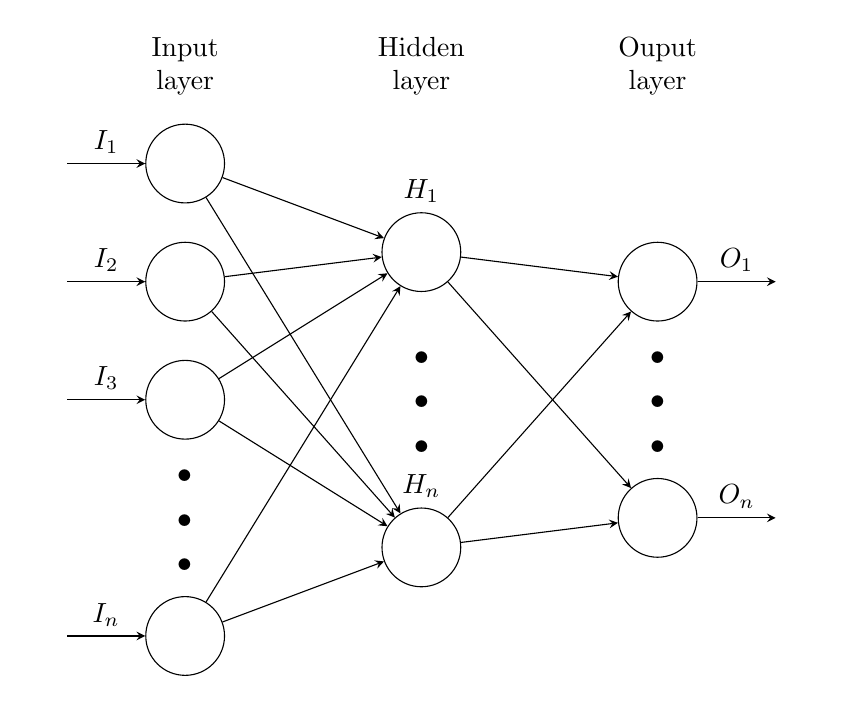
\begin{tikzpicture}[x=1.5cm, y=1.5cm, >=stealth]
		
		\foreach \m/\l [count=\y] in {1,2,3,missing,4}
		\node [every neuron/.try, neuron \m/.try] (input-\m) at (0,2.5-\y) {};
		
		\foreach \m [count=\y] in {1,missing,2}
		\node [every neuron/.try, neuron \m/.try ] (hidden-\m) at (2,2-\y*1.25) {};
		
		\foreach \m [count=\y] in {1,missing,2}
		\node [every neuron/.try, neuron \m/.try ] (output-\m) at (4,1.5-\y) {};
		
		\foreach \l [count=\i] in {1,2,3,n}
		\draw [<-] (input-\i) -- ++(-1,0)
		node [above, midway] {$I_\l$};
		
		\foreach \l [count=\i] in {1,n}
		\node [above] at (hidden-\i.north) {$H_\l$};
		
		\foreach \l [count=\i] in {1,n}
		\draw [->] (output-\i) -- ++(1,0)
		node [above, midway] {$O_\l$};
		
		\foreach \i in {1,...,4}
		\foreach \j in {1,...,2}
		\draw [->] (input-\i) -- (hidden-\j);
		
		\foreach \i in {1,...,2}
		\foreach \j in {1,...,2}
		\draw [->] (hidden-\i) -- (output-\j);
		
		\foreach \l [count=\x from 0] in {Input, Hidden, Ouput}
		\node [align=center, above] at (\x*2,2) {\l \\ layer};
		
	\end{tikzpicture}
	\caption{A simple structure of Radial Basis Function Neural Networks (RBFNN).}
\end{figure}

Suppose a continuous vector function, $F(Z)$, $\hat{F}(Z) = W^{T}S(Z)$, with $\hat{F}(Z)$ is the approximation of function $F(Z)$, where $Z$ is the input of neural networks vector, the optimal weight of neural networks being, $\hat{W} = [\hat{W}_{1}, \hat{W}_{2}, \hat{W}_{3}, \dots, \hat{W}_{n}] \in R^{nl}$, $S(Z) = [s_{1}(Z), s_{2}(Z), s_{3}(Z), \dots, s_{l}(Z)]$ is the regressor, and $l$ is the number of neurons. Going by the common use, with regressor being a Gaussian radical basis function:

\begin{align}
	s_{i} (||Z - u_{i}||) &= \boldsymbol{exp} \bigg[ \frac{-(Z-u_{i})^{T} (Z - u_{i})}{\sigma_{i}^{2}}\bigg] \\
	&u_{i}(i = 1, \dots, l) \text{ are distinct points in space}\nonumber \\
	&\sigma_{i} \text{ is the width of Gaussian membership function} \nonumber
\end{align}

This justify the ability of machine learning to improve itself, via concept of neurons and synapse connection bearing specific weight value for decisions that will allow the algorithm to give the best possible output to its extent (Jiang \etl, 2017; Mahmood \& Shrestha, 2019).

The number of value of weights, is then determined by the number of generations, or iteration, which is the number of exploration in the training data done by the algorithm, that reveals every possible pattern and correlation. The value of weight was then stored in neurons and synapses, and finally with enough iteration, the model can then determine the best path or connection of nodes for a certain task.

Thus it is concluded that machine learning algorithms are not in anyway conscious by itself, refuting the claims of artificial intelligence taking over the world, and poses an imminent threat to the human civilizations. Quoting mathematician and philosopher, Bertrand Russell, on his ``\textit{unyielding despair}'':

\begin{quote}
	That man is product of causes which had no prevision of the end they were achieving; that his origin, his growth, his hopes and fear, his loves and his beliefs, are but outcome of accidental collocation of atoms; that no fire, no heroism, no intensity of thought or feeling, can preserve a life beyond the grave; that all the labors of ages, all the devotion, all the inspiration, all the noon day brightness of human genius, are destined to extinction \dots
\end{quote}

Which was continued as ``\textit{by the vast death of galaxy}'', not ``\textit{by computers or artificial intelligence}'', as physicist Dr. Michio Kaku (1995) once echoed, ``\textit{a computer is nothing more than a sophisticated adding machine, an impeccable idiot.}''.

\newpage
\subsection*{Statement of the Problem\centering}

The study aims to implement a new system that replaces traditional methods, specifically the lock access, attendance checking, and security system, via the utilization of RFID technology and Arduino board, and machine learning models of face recognition. The study also sought to determine whether it can be utilized and successfully replace the traditional methods. Hence, in the final analysis the study sought to:

\begin{enumerate}
	\item Determine if RFID technology and Arduino board can be utilized as lock access system;
	\item Determine if machine learning models of face recognition can be utilized to check student's attendance, and as a security system;
	\item Devise a regression model of the cost-effectiveness of RFID and Arduino-based systems against traditional methods in the following time frame:
	\begin{enumerate}
		\item 12 months;
		\item 36 months;
		\item and 60 months;
	\end{enumerate}	
\end{enumerate}

\subsection*{Hypotheses of the Study\centering}

The researchers devised the following null hypotheses to be disproved by the study:

\begin{enumerate}
	\item RFID technology and Arduino board are not suitable to be utilized as lock access system;
	\item Machine learning models of face recognition are not compatible for utilization to check the attendance of students and as a security system.
	\item RFID and Arduino-based lock access systems are less cost efficient than traditional methods in the following time frame:
	\begin{enumerate}
		\item 12 months;
		\item 36 months;
		\item and 60 months;
	\end{enumerate}
\end{enumerate}

\subsection*{Objectives of the Study\centering}

It is necessary to guarantee and provide the safety and security of students in school successfully. Moreover, due to the exponential improvement of technology (Kaku, 1995), adapting to the changes is a necessity as it did not only created a new path for opportunities, but also increases the number and acceleration of threat, thus the study aims to implement the technological advancements to deal with and resist the infringement on security and privacy as well as its exploitation. Therefore, the objectives of the study are:

\begin{enumerate}
	\item Implement the current technological advancement for use in long term use.
	\item Develop a \textit{de novo} convenient and efficient system as a replacement of traditional lock access, attendance checking, and security system.
	\item Utilize RFID technology and Arduino board, and machine learning models of face recognition for use in locker, and attendance and security system, respectively.
\end{enumerate}

\subsection*{Significance of the Study\centering}

The interconnectivity of every organism (Lewin \etl, 2018; Lewin \etl, 2022) relays the changes and actions of one to another, thus a change in one society will affect another and may even affect larger systems, which is also known as butterfly effect in Chaos theory. Hence, making the correct action may likely lead to improvement of the particular society at the very least, while making the opposite may lead to acceleration of depressing consequence or the ``\textit{unyielding despair}'', once echoed by mathematician and philosopher, Bertrand Russell (Kaku, 1995).

Among the goals of the study is to address the gap and vulnerability of currently implemented mechanisms and technology of traditional methods via utilization and implementation of RFID technology and Arduino board, and machine learning models of face recognition as replacement of the inefficient traditional and other methods in current use, specifically lock access, and attendance checking and security system, respectively.

\textbf{School Administrators}. This study will help the school administrators to ascertain that the basic rights of students are provided. It would also help in improving comfort, in sense of security, and convenience. Moreover, the study would significantly decrease the cost in maintenance, as well as the implementation and replacement, and the overall expenses in macro scale, thus allowing the funds to be utilized in other necessities, and help in adaptation and transition for the other upcoming innovations and technological revolutions.

\textbf{Students}. This study will ensure the safety and privacy of students within the school area, due to the decreased entry and simplified reporting as well as alert of break in by intruders, or other unregistered entities. Furthermore, the RFID and Arduino-based lock access systems, are more robust in providing security to the lockers, and other storage rooms, thus ensuring the security of belongings of students.

\textbf{Parents and teachers}. The sense of comfort the study would provide due to the assurance of safety of students, would give a significant relief in parents and teachers. Furthermore, in long term, the study would decrease the costs expended in utilities such as attendance notebooks.

\textbf{Environment, and general community}. The study also significantly reduces the use of other materials such as locks, and attendance notebooks in macro scale, thus decreasing the contribution for increasing solid wastes, that further contributes to pollution.

\subsection*{Scope and Delimitation\centering}

The study was limited in devising an RFID and Arduino-based lock access systems, and face recognition-based attendance checking and security systems derived from machine learning models of face recognition, as one of the main goals of the study is to utilize and implement the current technological advancements.

The models of RFID and Arduino-based lock access systems and face recognition-based attendance checking and security systems was evaluated in terms of unlock and lock time, and classification time as well as classification ability, respectively. While for face recognition-based attendance checking and security systems derived from machine learning models of face recognition, a complete software was created by the researchers, with a fully functioning algorithm that can be further imported as module for other purposes, and modified as per certain needs.

A \texttt{git} repository with complete branches and code commits  history with complete description of changes were also provided for further studying of the source code, including the example database as one of the branches with template for production-ready utilization.

Linear regression models of with time frames of 12 months, 36 months and 60 months were also devised to model the cost efficiency of Arduino against traditional methods. 

\subsection*{Theoretical Framework\centering}

Machine learning, also known as computational learning theory, is a subset of artificial intelligence that has the ability of to improve itself through repeated iteration on previous and new datasets (Mahmood \& Shrestha, 2019) that allows for discovery of new patterns and correlations of the variables, improving the neural networks (Jiang \etl, 2017; Mahmood \& Shrestha, 2019). Avrim Brum, from Carnegie Mellon University, further defined it as an ability of the algorithm to improve itself and learn from new inputs and adapt to changes, which improves the performance through ``\textit{experience}''. By doing so, machine learning algorithms can predict and simulate phenomena based on the previous dataset or random inputs from curated dataset, moreover, depending on the model type, it is also possible to produce \textit{de novo} outputs from the algorithm.

\subsection*{Conceptual Framework\centering}

\begin{figure}[h!]
	\centering
	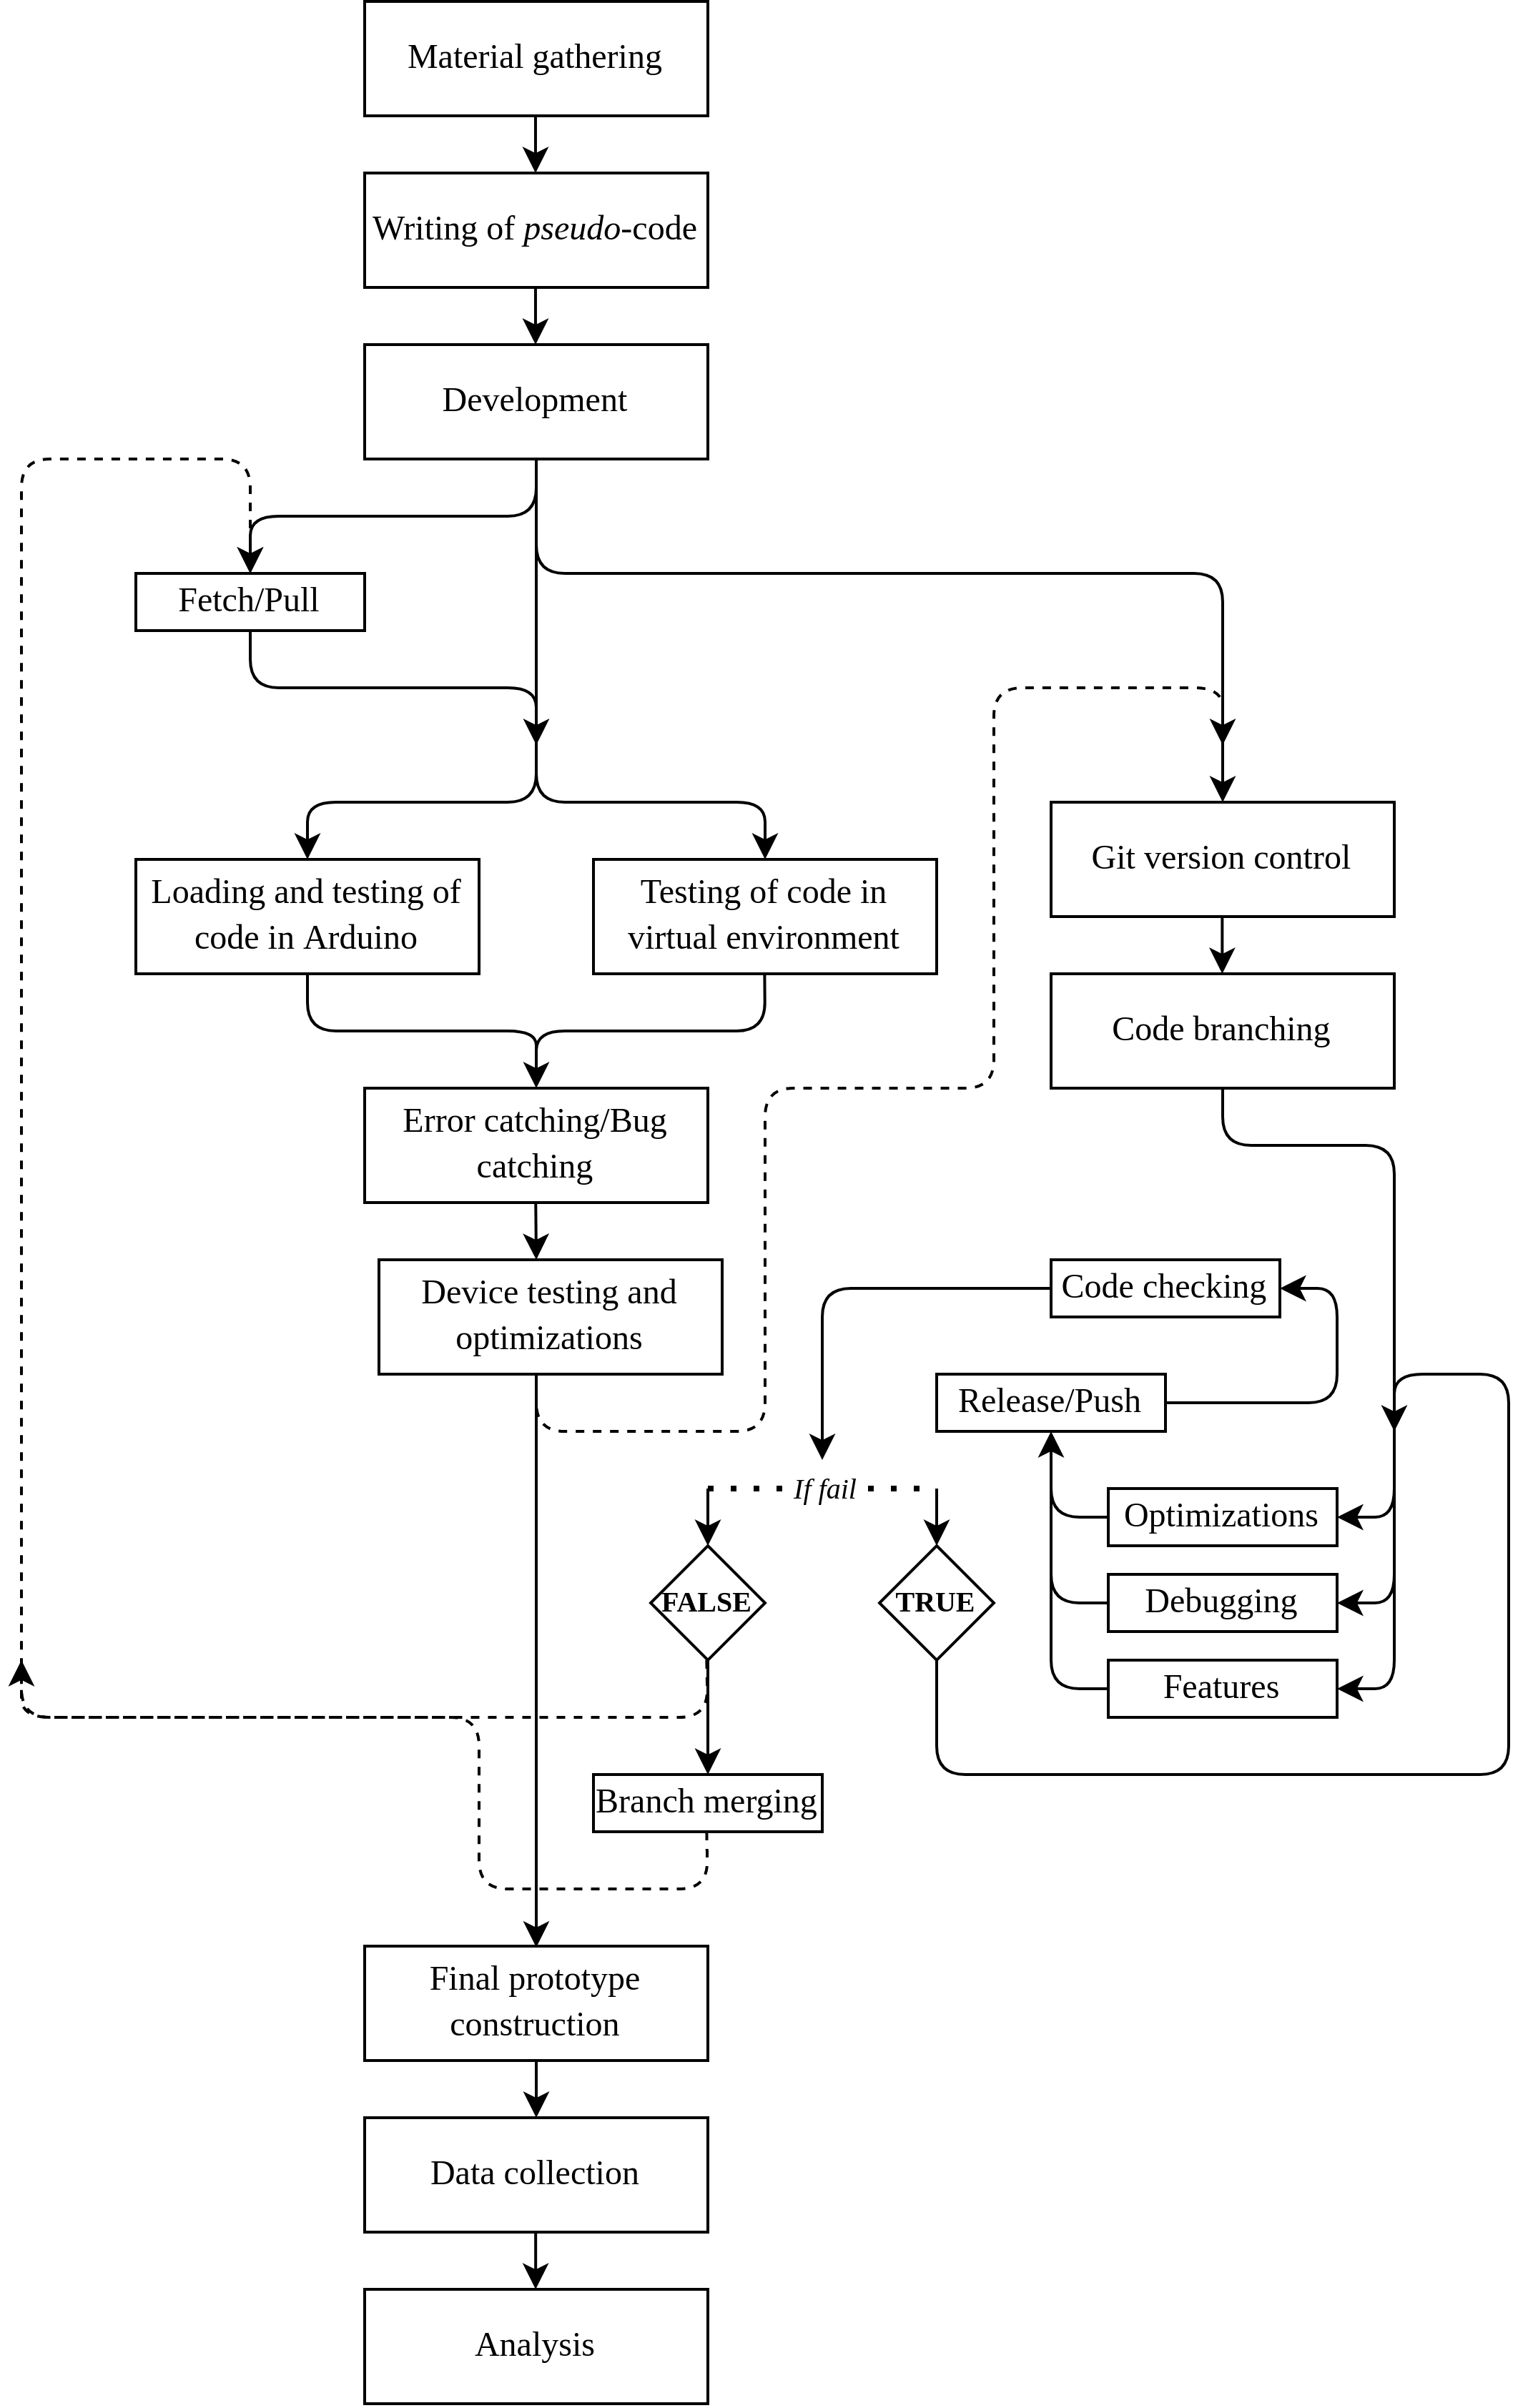
\includegraphics{cframework.png}
	\caption{Conceptual framework of the study.} \label{fig:1}
\end{figure}

The series are broken into 3 phases, the first phase is the preparation, this includes the gathering of the materials needed in the study, and the writing of \texttt{pseudo}-code, as well as its pre-writing.

After the code is prewritten, various branch was created per certain point in milestone for (1.) implementation of new features; (2.) optimizations of code base; (3.) and debugging, marking the start of phase 2. The code of lock access algorithm was then loaded into Arduino, while the machine learning models of face recognition was executed inside virtual environment for testing, optimizations, and error and bug catching. In this phase, all of noticed and caught bugs were fixed in its respective code branch, which was assessed by Codiga, an artificial intelligence assessment utility for code repositories, per pull request for (1.) compliance to Python's Enhancement Proposals (PEP), as well as suggestions of various linters such as PyLint, which was defined as rules, namely: \texttt{E0\emph{XXX}}, \texttt{R*\emph{XXX}}, \texttt{C*\emph{XXX}}, \texttt{W\emph{XXX}}, \texttt{B[1-2]\emph{XXX}}, \texttt{I.\emph{XXX}}, categorized per severity as (1.) error; (2.) warning; (3.) security; (4.) and informational. If the code of the pull request violated the rules, the pull request should be fixed with another commit(s) in addition to the existing pull request. The changes from code branch then would be pulled and loaded again for further testing, and error and bug catching. Depending on the case, the branch can then be merged or further forked. The process was done repeatedly until there were no noticeable bugs in the end user perspective, has a considerable execution speed, and smooth performance of program. Finally, the all the conflicts per code branch were fixed, and then branches of the code were merged with the main branch.

In the final phase, the final prototype was constructed, and had undergone data collection. The data was then analyzed using \texttt{pandas}, \texttt{statistics}, and visualized using \texttt{matplotlib}.

\subsection*{Definition of Terms\centering}

\textbf{Branch} – is copy of the specified code branch.

\textbf{Character (\texttt{char})} - is a data type that strictly includes only one ASCII.

\textbf{Commit} - the addition of change in code base for the next push, which is done after the staging of changes. 

\textbf{Container} – is an isolated \textit{pseudo}-operating system (OS) used for experimental purposes, such as testing and simulation to avoid main production system pollution.

\textbf{Merge} – is the combining of two different branches, if the pull request was accepted.

\textbf{Modules} – are external code library files, with a suffix of \texttt{.py} for a Python code, that contains the additional piece for a particular software.

\textbf{Push} – is the sending of changes from \texttt{origin} to the \texttt{git} repository.

\textbf{Pull} – process of fetching the new changes from the \texttt{git} repository to the cloned branch.

\textbf{Origin} - the source of the upcoming commits for a particular \texttt{git} repository.

\textbf{String} (\texttt{S|string})- is a data type consisted of more than one character.

\newpage
\section*{METHODOLOGY\centering}

This chapter presents the complete description of all procedures. 

\subsection*{Materials\centering}

The main materials used in the study are 1 Arduino UNO R3 board, 20 jumper wires (mm, mf), 1 MFRC522 RFID card reader, 2 RFID cards, 1 $27 \times 4$ 12C LCD screen, 1 servo motor, 9V snap power to DC plug, and 9V battery,

Other materials used are plywood, wood filler, sticker and handle. Electric drill, saw, philips head screws, were also used for creation of the locker prototype.

There were no materials used in machine learning models of face recognition model. An input camera, and faces as training data, is required, however, which includes a myriad of diverse faces.

\subsection*{Procedures\centering}

\subsubsection*{Device Engineering}

The lock access, attendance checking, and the security system, has the same input process. The systems take input data to be compared from references in database or system itself, which will be taken from a real-time input device, specifically MFRC522 card reader for lock access, and camera for attendance checking and security system.

In RFID and Arduino-based lock access systems, the receiver takes the information or the 10 character-length string datatype Unique IDentifier (UID) of the RFID card and relayed to the Arduino, while in face recognition-based attendance checking and security systems the camera takes the frame from a video feed, and relay it to the algorithm. However, it differs significantly in the process of systemically verifying and checking the information received.

The RFID and Arduino-based lock access checks the UID using the string compare algorithm loaded in the board, written in C++20. On contrary to the machine learning face recognition-based attendance checking and security system, whereas it needs a large database of students and teachers information, and intensive process, it requires the use of \texttt{x86\_64} or \texttt{amd64} system. The input taken from the camera, was then relayed to the checking algorithm written in Python 3.10.4.

\subsection*{Software Engineering}

\subsubsection*{\emph{RFID and Arduino-based Lock Access System Algorithm}}

The algorithm of the RFID and Arduino-based lock access system was depicted by Figure 5, which was written in C++20, and loaded to the board.

\begin{figure}[h!]
	\centering
	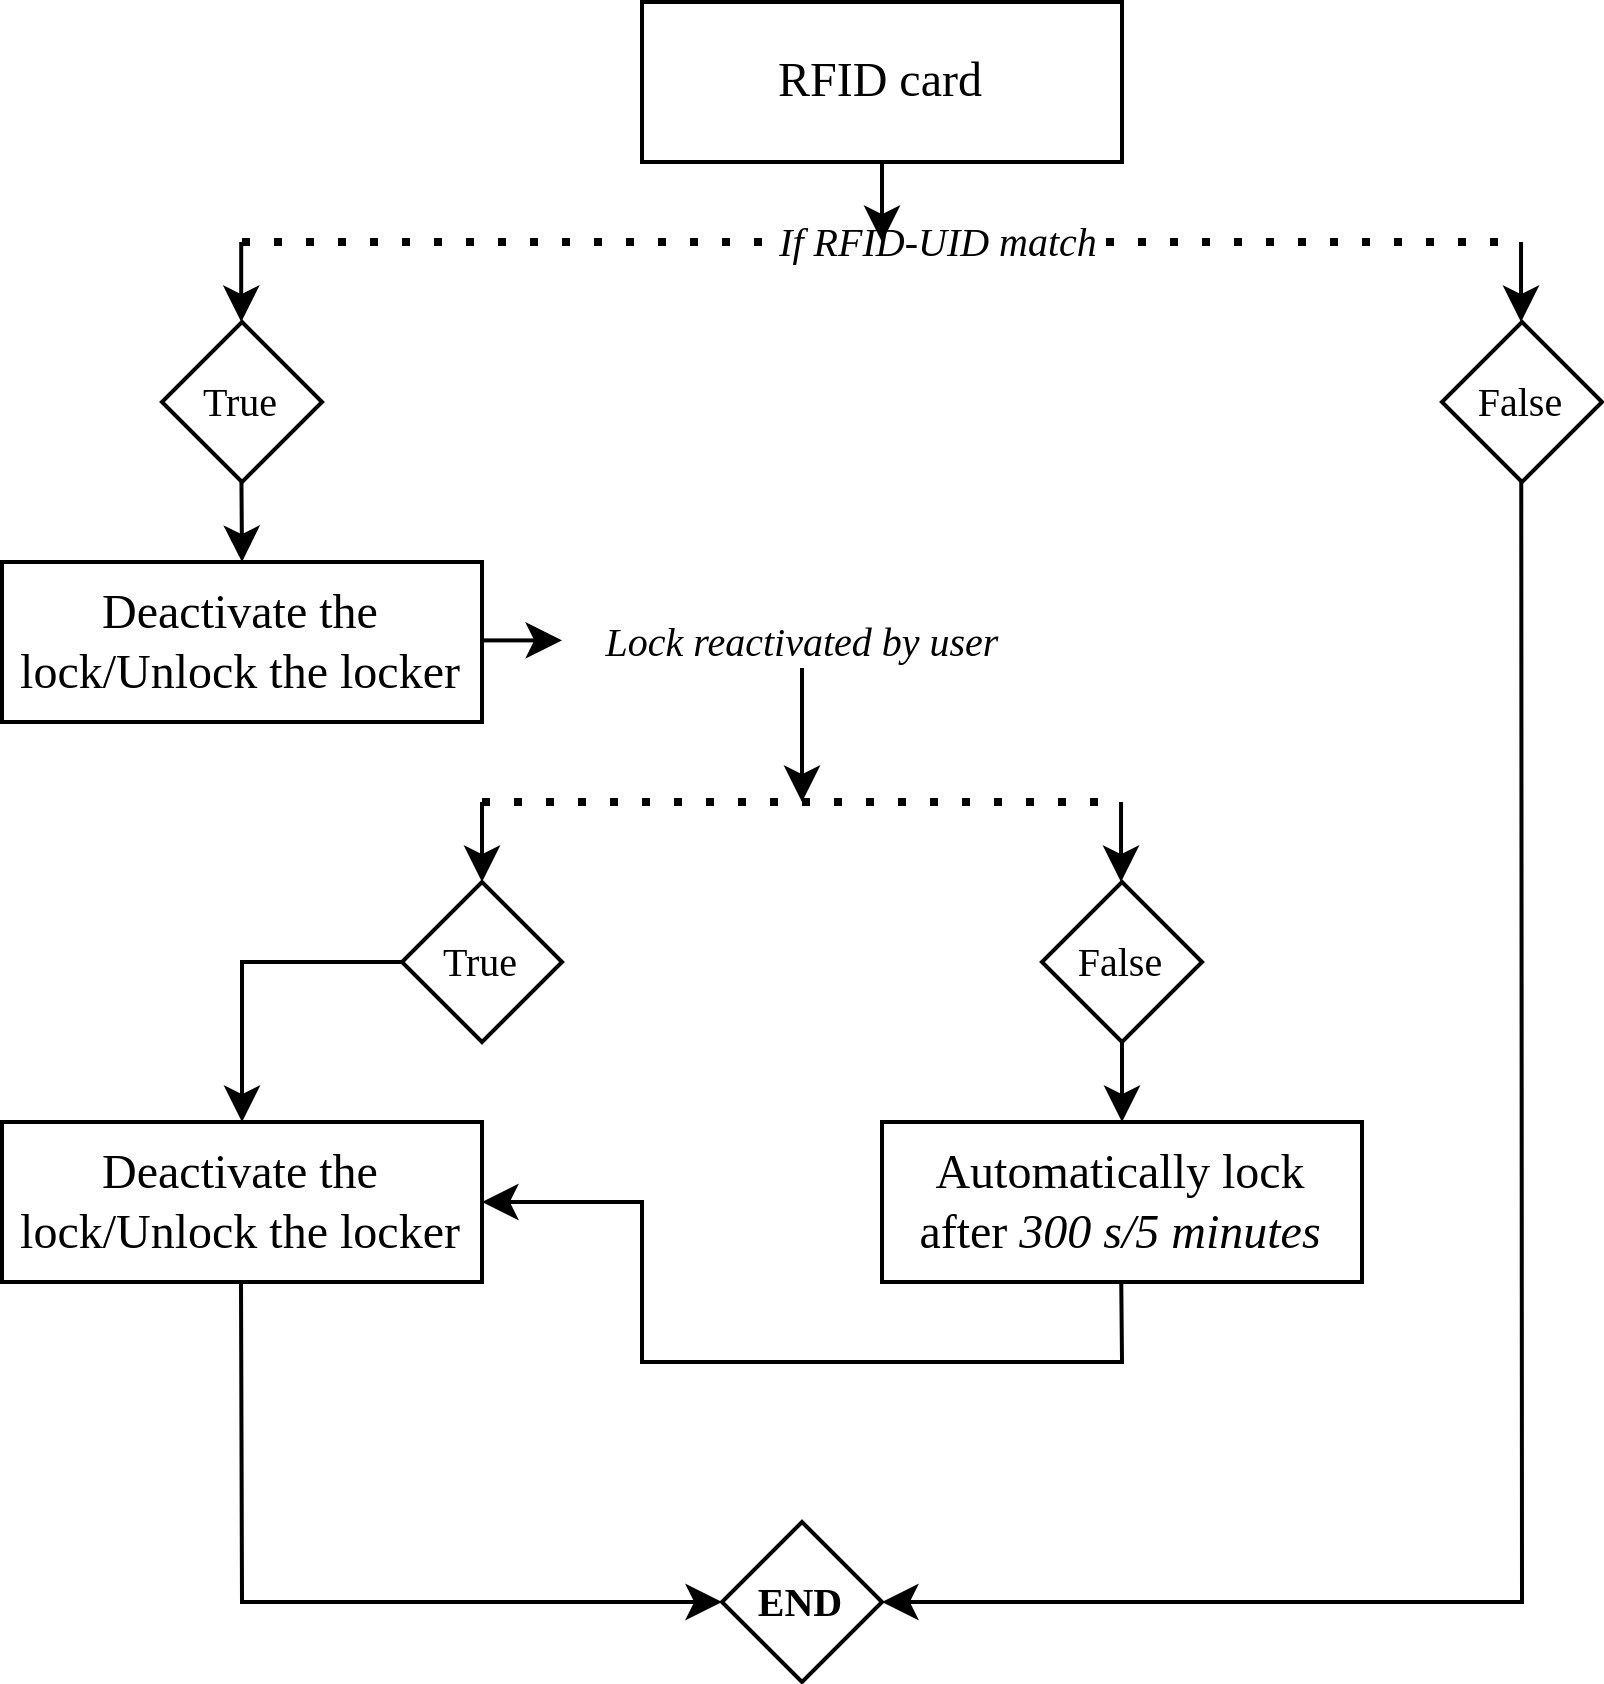
\includegraphics{fig_locker.png}
	\caption{RFID and Arduino-based lock access system algorithm.}
\end{figure}

To check the input UID from reference UID stored as \texttt{String} datatype, the algorithm compares the \texttt{hexdump} or hexadecimal view of the two string, the reference UID, and the input UID, from memory:

\singlespacing
\begin{lstlisting}[language=bash, caption={Example of hexadecimal view of various strings}]
# string "hello"
$ echo "hello" | hexdump
0000000 6568 6c6c 0a6f                         
0000006

# string "Hello"
$ echo "Hello" | hexdump
0000000 6548 6c6c 0a6f                         
0000006

# string "GH 5H 7Y 8U"
$ echo "GH 5H 7Y 8U" | hexdump
0000000 4847 3520 2048 5937 3820 0a55          
000000c

# string "GH 5H 8U 7Y"
$ echo "GH 5H 8U 7Y" | hexdump
0000000 4847 3520 2048 5538 3720 0a59          
000000c
\end{lstlisting} 
\doublespacing

This returns the hexademical view of the input string, which will be compared from the reference string stored in the system. With the results, it is apparent that the string \texttt{Hello} is different from \texttt{hello}, as well as \texttt{GH 5H 8U 7Y} and \texttt{GH 5H 7Y 8U}. Using the hexadecimal view of the string, the algorithm can determine and successfully compare the input UID from reference UID.

\subsubsection*{\emph{Face Recognition-based Attendance and Security System}}

The main algorithm, as shown in the Figure 6, of the system was written in Python 3.10.4 with the student database stored locally as JavaScript Object Notation (JSON) file (refer to Listing 2), and synchronized with the online repository via \texttt{git} using \texttt{systemd} service.

\begin{figure}[h!]
	\centering
	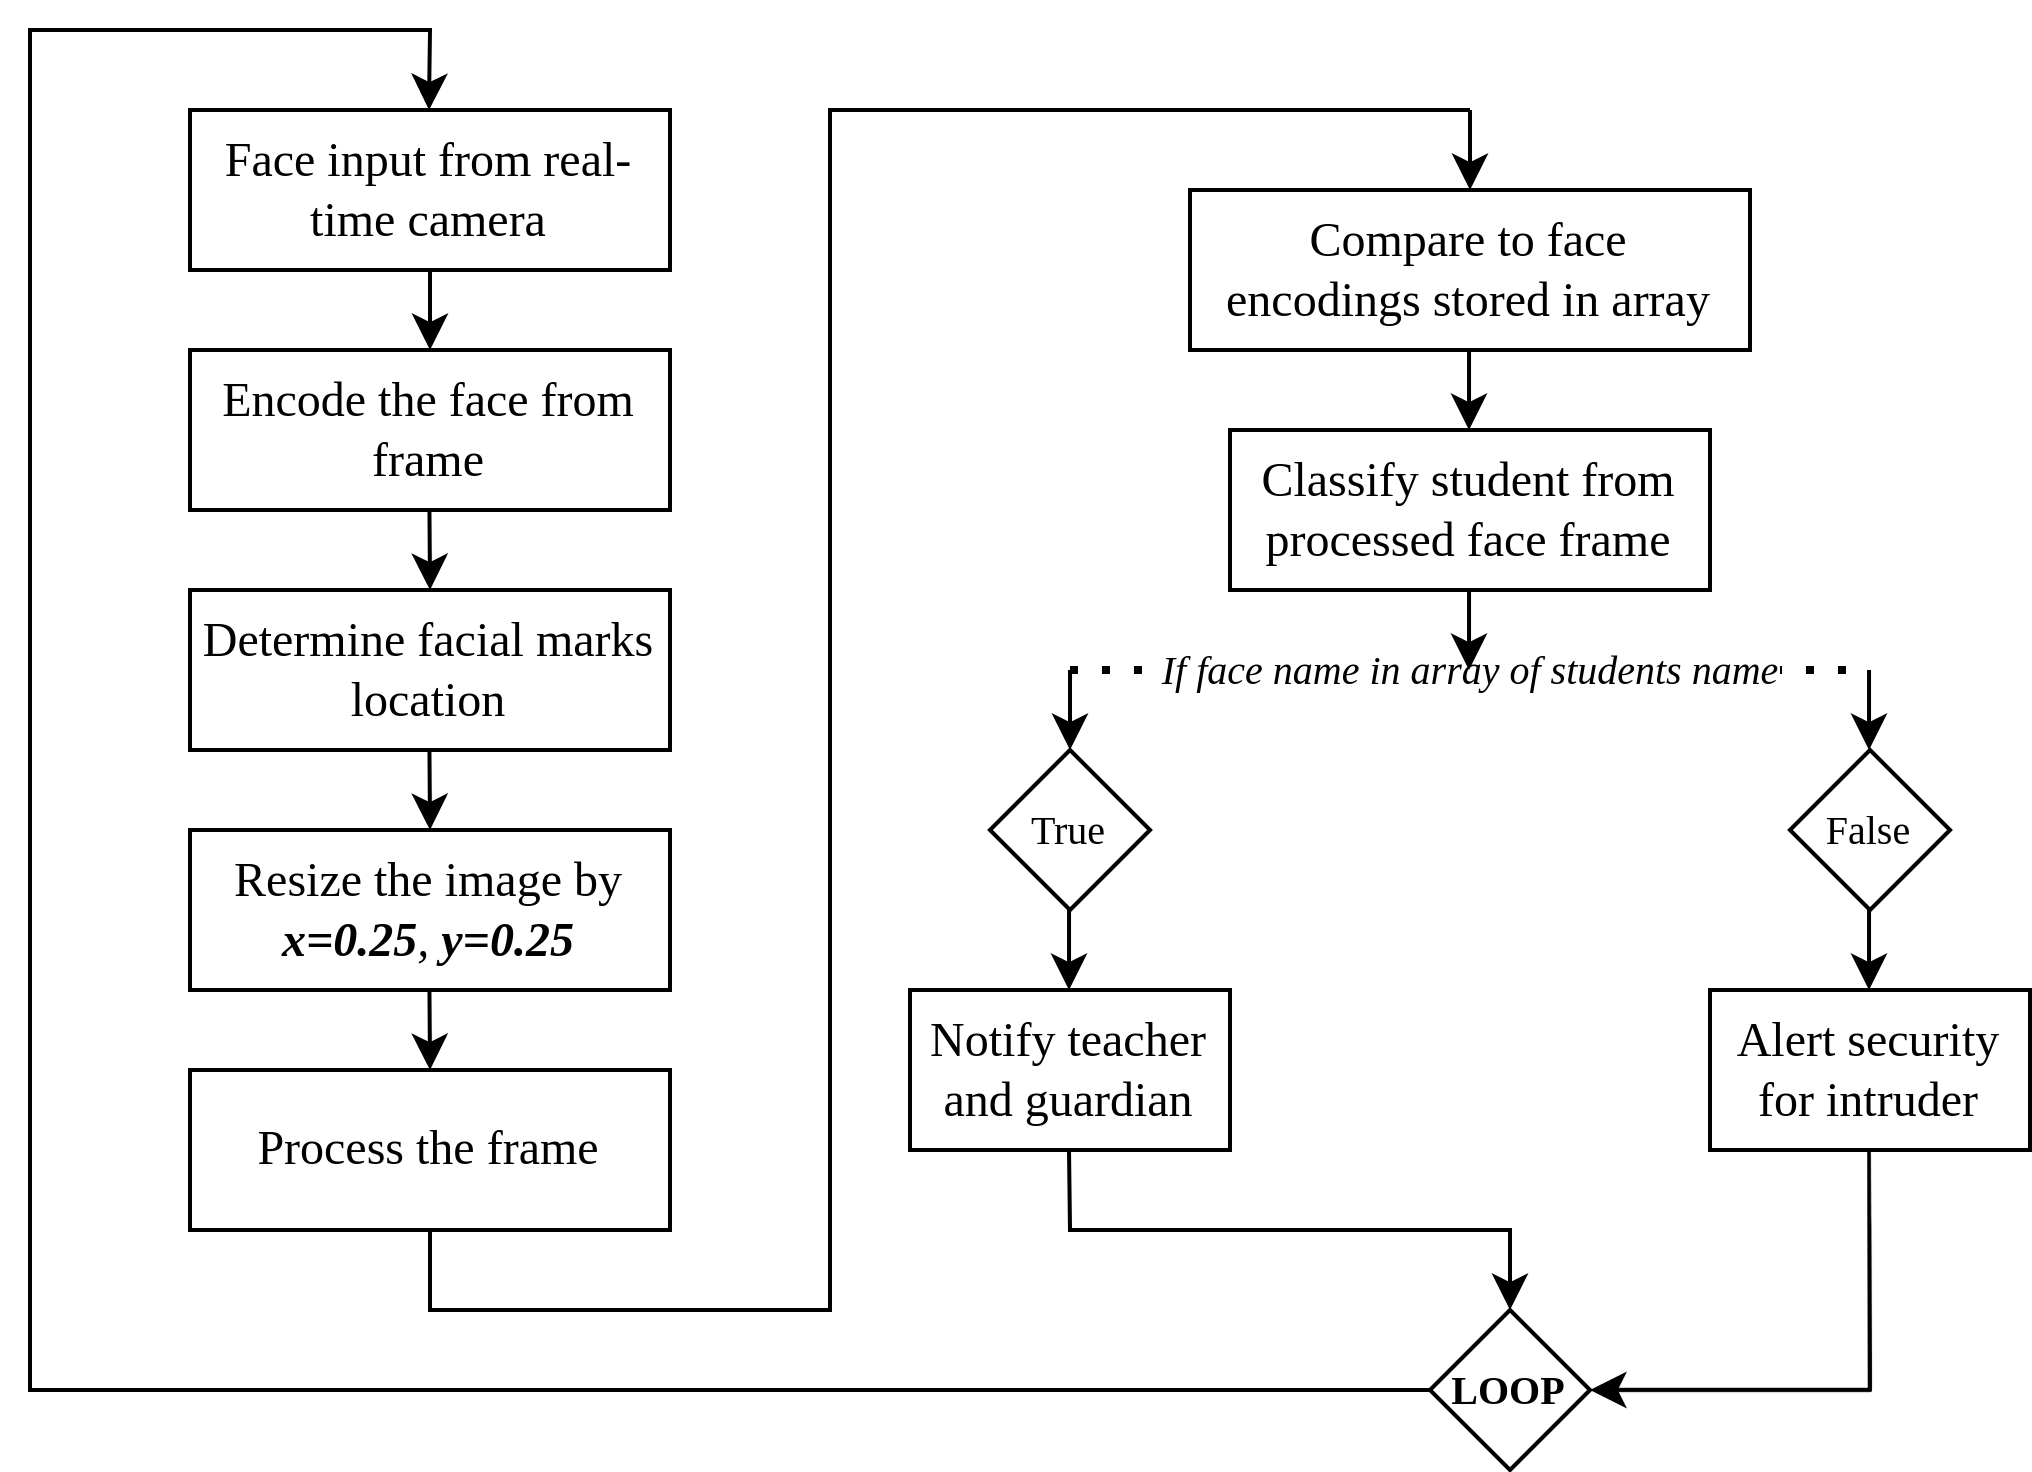
\includegraphics{fig_fr.png}
	\caption{Algorithm of face recognition-based attendance checking and security system.} \label{fig:4}
\end{figure}

\singlespacing
\begin{lstlisting}[language=Python, caption={Example of stored student information in database.}]
{
	
	"Nicole Amber Hennessey": [
		"std1.png",
		"12 STEM - Fleming",
		"Menard Miguel",
		"Melody Hennesey",
	],
	
	"Raven Gose": [
		"std2.png",
		"12 STEM - Fleming",
		"Menard Miguel",
		"Venifer Gose",
	],	
	
	"Fiona Leigh Pagtama": [
		"std3.png",
		"12 STEM - Fleming",
		"Menard Miguel",
		"Emeriza Pagtama",
	],
	
	"Student n" : [
		"std<n>.png",
		"<section>",
		"<adviser>",
		"<legal guardian>",
	]
	
	...,

}
\end{lstlisting}
\doublespacing

Various third party modules were used to aid the Python standard library for successful execution of the function. A pre-trained machine learning model was utilized and implemented by the researchers, \texttt{face\_recognition==1.3.0} based from \texttt{dlib} (\texttt{python3-dlib.fc36*}), while \texttt{numpy==1.22.3} was used to provide the needed mathematical calculation to determine the face locations, and assist in the frame processing, and \texttt{opencv-python==4.5.5.64} to access the camera feed, and further frame processing. The email was composed using \texttt{email.message.Email.Message} and sent using Python's \texttt{smtplib}, and \texttt{ssl}, Simple Mail Transfer Protocol, and Secure Sockets Layer, respectively, in addition to \texttt{socket}.

Other modules utilized are \texttt{json} for parsing of the student data stored as JSON, \texttt{sys} and \texttt{os} for executing of kernel commands, \texttt{rich.console.Console==12.4.1} to give an informative \texttt{stdout} of the program, \texttt{argparse} was used to design the commandline interface (CLI), \texttt{random} to generate of \textit{pseudo}random ASCII characters imported from \texttt{string} for secure access of the database, and \texttt{geocoder==1.38.1} to track the IP address of the computer. \texttt{git} repository was also setup to be able to modify the data through graphical interface, that will be pulled every 24 hours by a defined \texttt{systemd} service.

The algorithm first locates the data of students in database with \texttt{os.path.expanduser()}. After successful location, \texttt{json} will parse the data of the students, and store it in high dimensional array with size of $N$, and the array inside with size of $M$. The images was then loaded with \texttt{face\_recognition.load\_image\_file()},  and encoded using \texttt{face\_recognition.face\_encodings()}, then was stored in a single dimensional array with size of $J$, as reference(s).

As depicted by the figure above, the program takes input from real-time camera accessed using \texttt{cv2.VideoCapture(x)} function from \texttt{opencv-python}, which was encoded by \texttt{face\_recognition} module. To verify the input faces, the algorithm locates the facial features of the frame taken from the input, to decrease the processing time, the input frame were resized by $-25\%$, in dimensions of $x$ and $y$ using \texttt{numpy}, and was recolored using \texttt{opencv-python}. After processing, the frame was encoded with the same function. Then, it compares the processed input frame encoding, with the encodings of faces stored inside array of size $N$, via repeated iteration, until a face was matched, or the sequence was completed:

\begin{figure}[h!]
	\centering
	\includegraphics{for\_loop.png}
	\caption{Comparison of encoded frame against encoded references in array.}
\end{figure}

After confirmed match, the algorithm will send an email to the (1.) registered guardian of the student; and (2.) class adviser of the student including the information of (1.) student; (2.) section; and (3.) time of attendance. If an unrecognized face is detected, on the other hand, an alert email would be sent to the registered security personnel.

\section*{Statistical Treatment and Analysis\centering}

To study the cost efficiency of the Arduino-based systems, a regression model was devised. Where the algorithm will learn the hypothesis, $\mathbf{h}$ using the existing given data set that it can be used to predict $\boldsymbol{y_i}$ using $\boldsymbol{x_i}$ and the parameters of the hypothesis, $\theta_1, \theta_2, \dots, \theta_n$, in an equation form of: 

\begin{equation}
	h_\theta (\boldsymbol{x_i}) = \theta_n + \theta_o (\boldsymbol{x_i})
\end{equation}

The regression model devised includes a time frames of 12 months, 36 months, and 60 months, based on the previous fluctuation of prices of Arduino from March 03, 2021 to May 17, 2022 from records of \href{pricehistory.in}{https://pricehistory.in/s/SZ\_0E}. The data was used to initially generate the set of $\boldsymbol{x_i}$ and $\boldsymbol{y_i}$, which was further used to generate the new generation data.

Then the generated items from data was further processed with Equation 27:

\begin{align}
	\boldsymbol{x_i} &= \frac{\mathbb{R}(dataset_{n})^{\boldsymbol{ln}(\mathbb{R}(dataset_{n}))}}{\mathbb{R}(dataset_{n})+\mathbb{R}(datasest_{n})}
\end{align}	

And finally, was subjected to linear regression.

\newpage
\section*{PRESENTATION AND INTERPRETATION OF RESULTS\centering}

This project was conducted in order to determine whether RFID technology and Arduino board, and machine learning models of face recognition can be utilized and implemented as lock access, and attendance checking and security system, respectively.

\subsection*{Research Findings\centering}
\subsubsection*{RFID and Arduino-based Lock Access System}

\begin{figure}[h!]
	\centering
	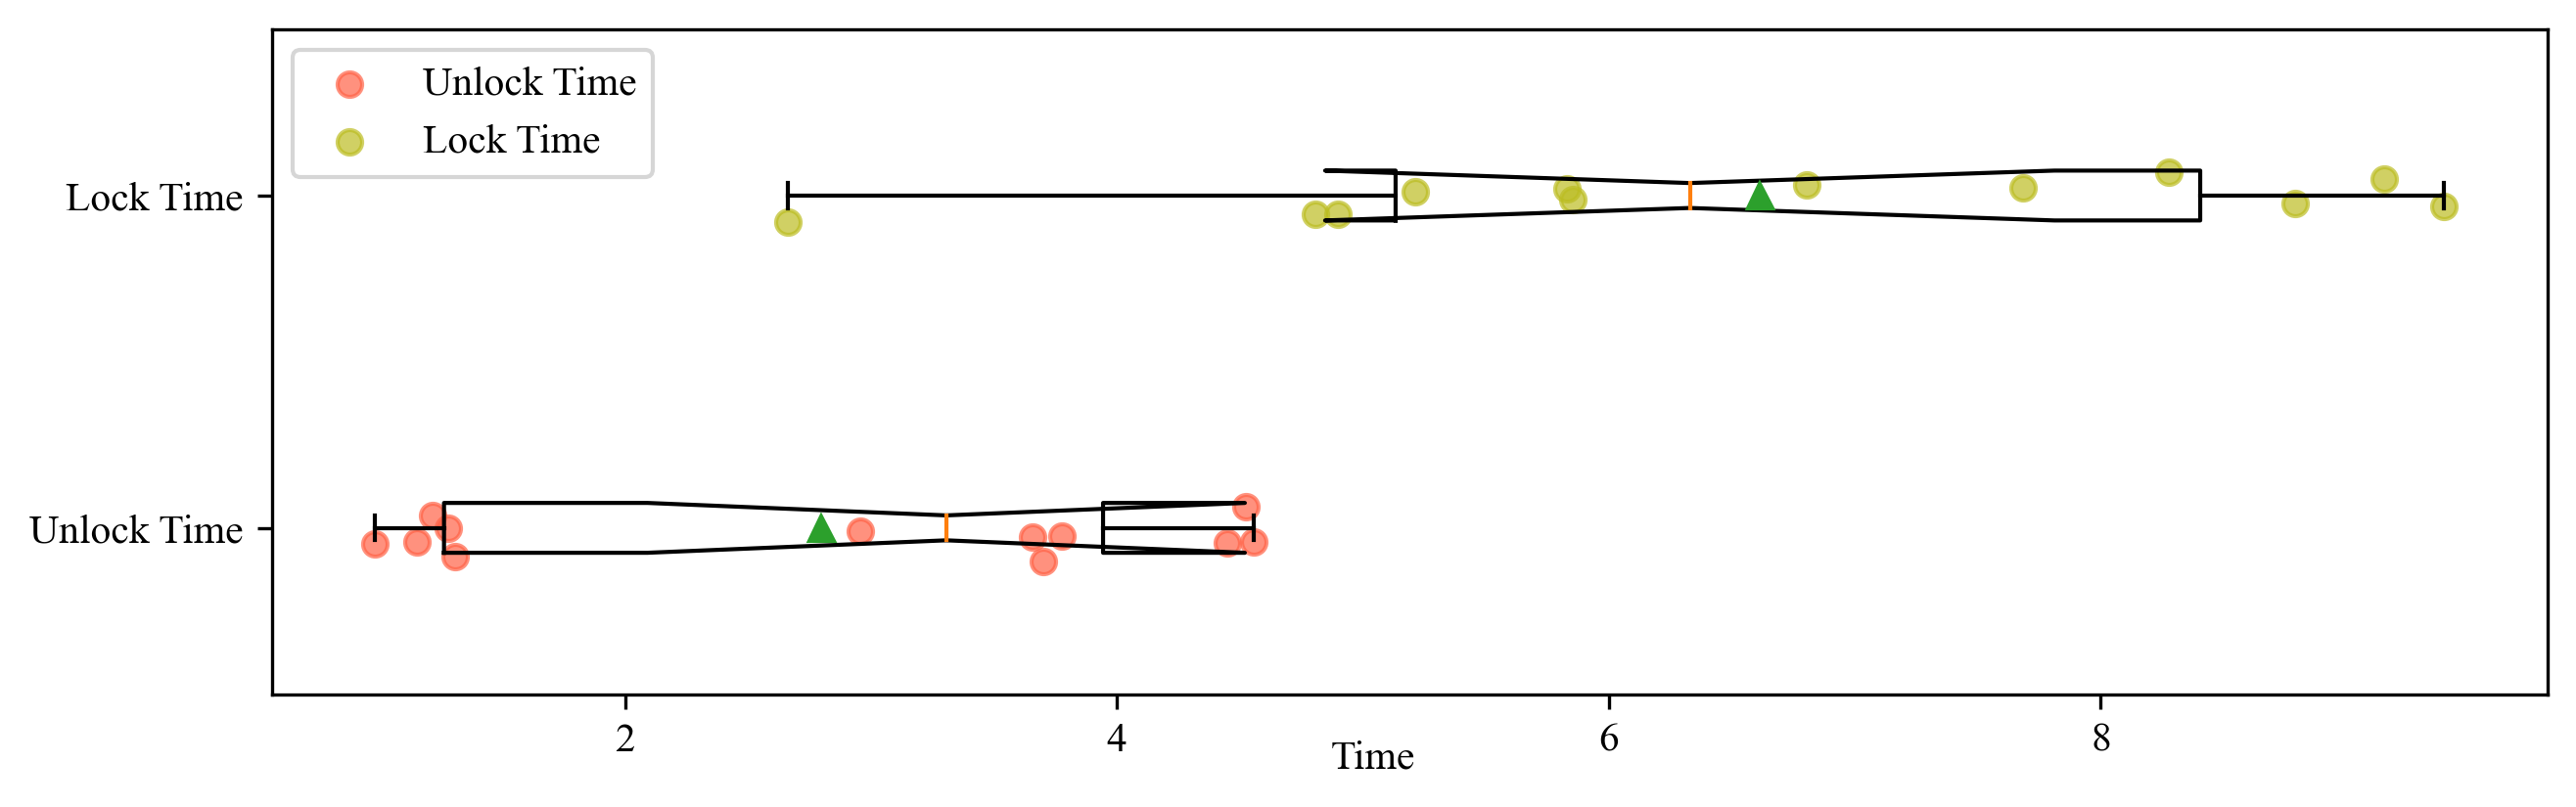
\includegraphics[width=\textwidth]{fig_1da1.png}
	\caption{Unlock and lock times of RFID and Arduino-based lock access systems.}
\end{figure}

According to the measurements conducted, the RFID and Arduino-based lock access system, have an average of $\mu_{t_{unlock}} = 2.797147062378335s \longrightarrow 2.80s \pm 0.10s$ for unlock time, and $\mu_{t_{lock}} = 6.613831762216549s \longrightarrow 6.60s \pm 0.10s$, as shown by 12 trials in Figure 8. Compared to traditional access methods, such as padlocks, which uses different lock systems such as pin, among others, or a standard doorknob with keys, that may take up to $5s < \mu_{t}$.

Moreover, the hidden lock system of the RFID and Arduino-based lock access systems render the common forms of lock bypassing methods useless, and the string compare algorithm also further decreases the vulnerability of the system, since a 10 character-length string contains a significantly different checksum than other UID, as shown by Listings 1. This decreases the hacking vulnerability of the system. Thus an RFID and Arduino-based lock access systems, provides more robust and secure system, compared to the traditional lock access systems.

Furthermore, it should also be considered that the performance of the system can further be improved, considering the compromisation of speed due to the high latency time of the LCD display and the module for its access, \texttt{<LiquidCrystal\_I2C.h>}, as well as the delay caused by other functions particularly by \texttt{<Chrono.h>} that provides \texttt{.hasPassed(time)} function for the countdown functionality, and the \texttt{<Servo.h>} module that facilitates the control of servo motors used in the locking. Suggesting that the models, despite not in best possible performance, yields an average response time of $\mu_t = 4.7s \pm 0.10s$.

\subsubsection*{Face Recognition-based Attendance Checking and Security System}

\begin{figure}[h!]
	\centering
	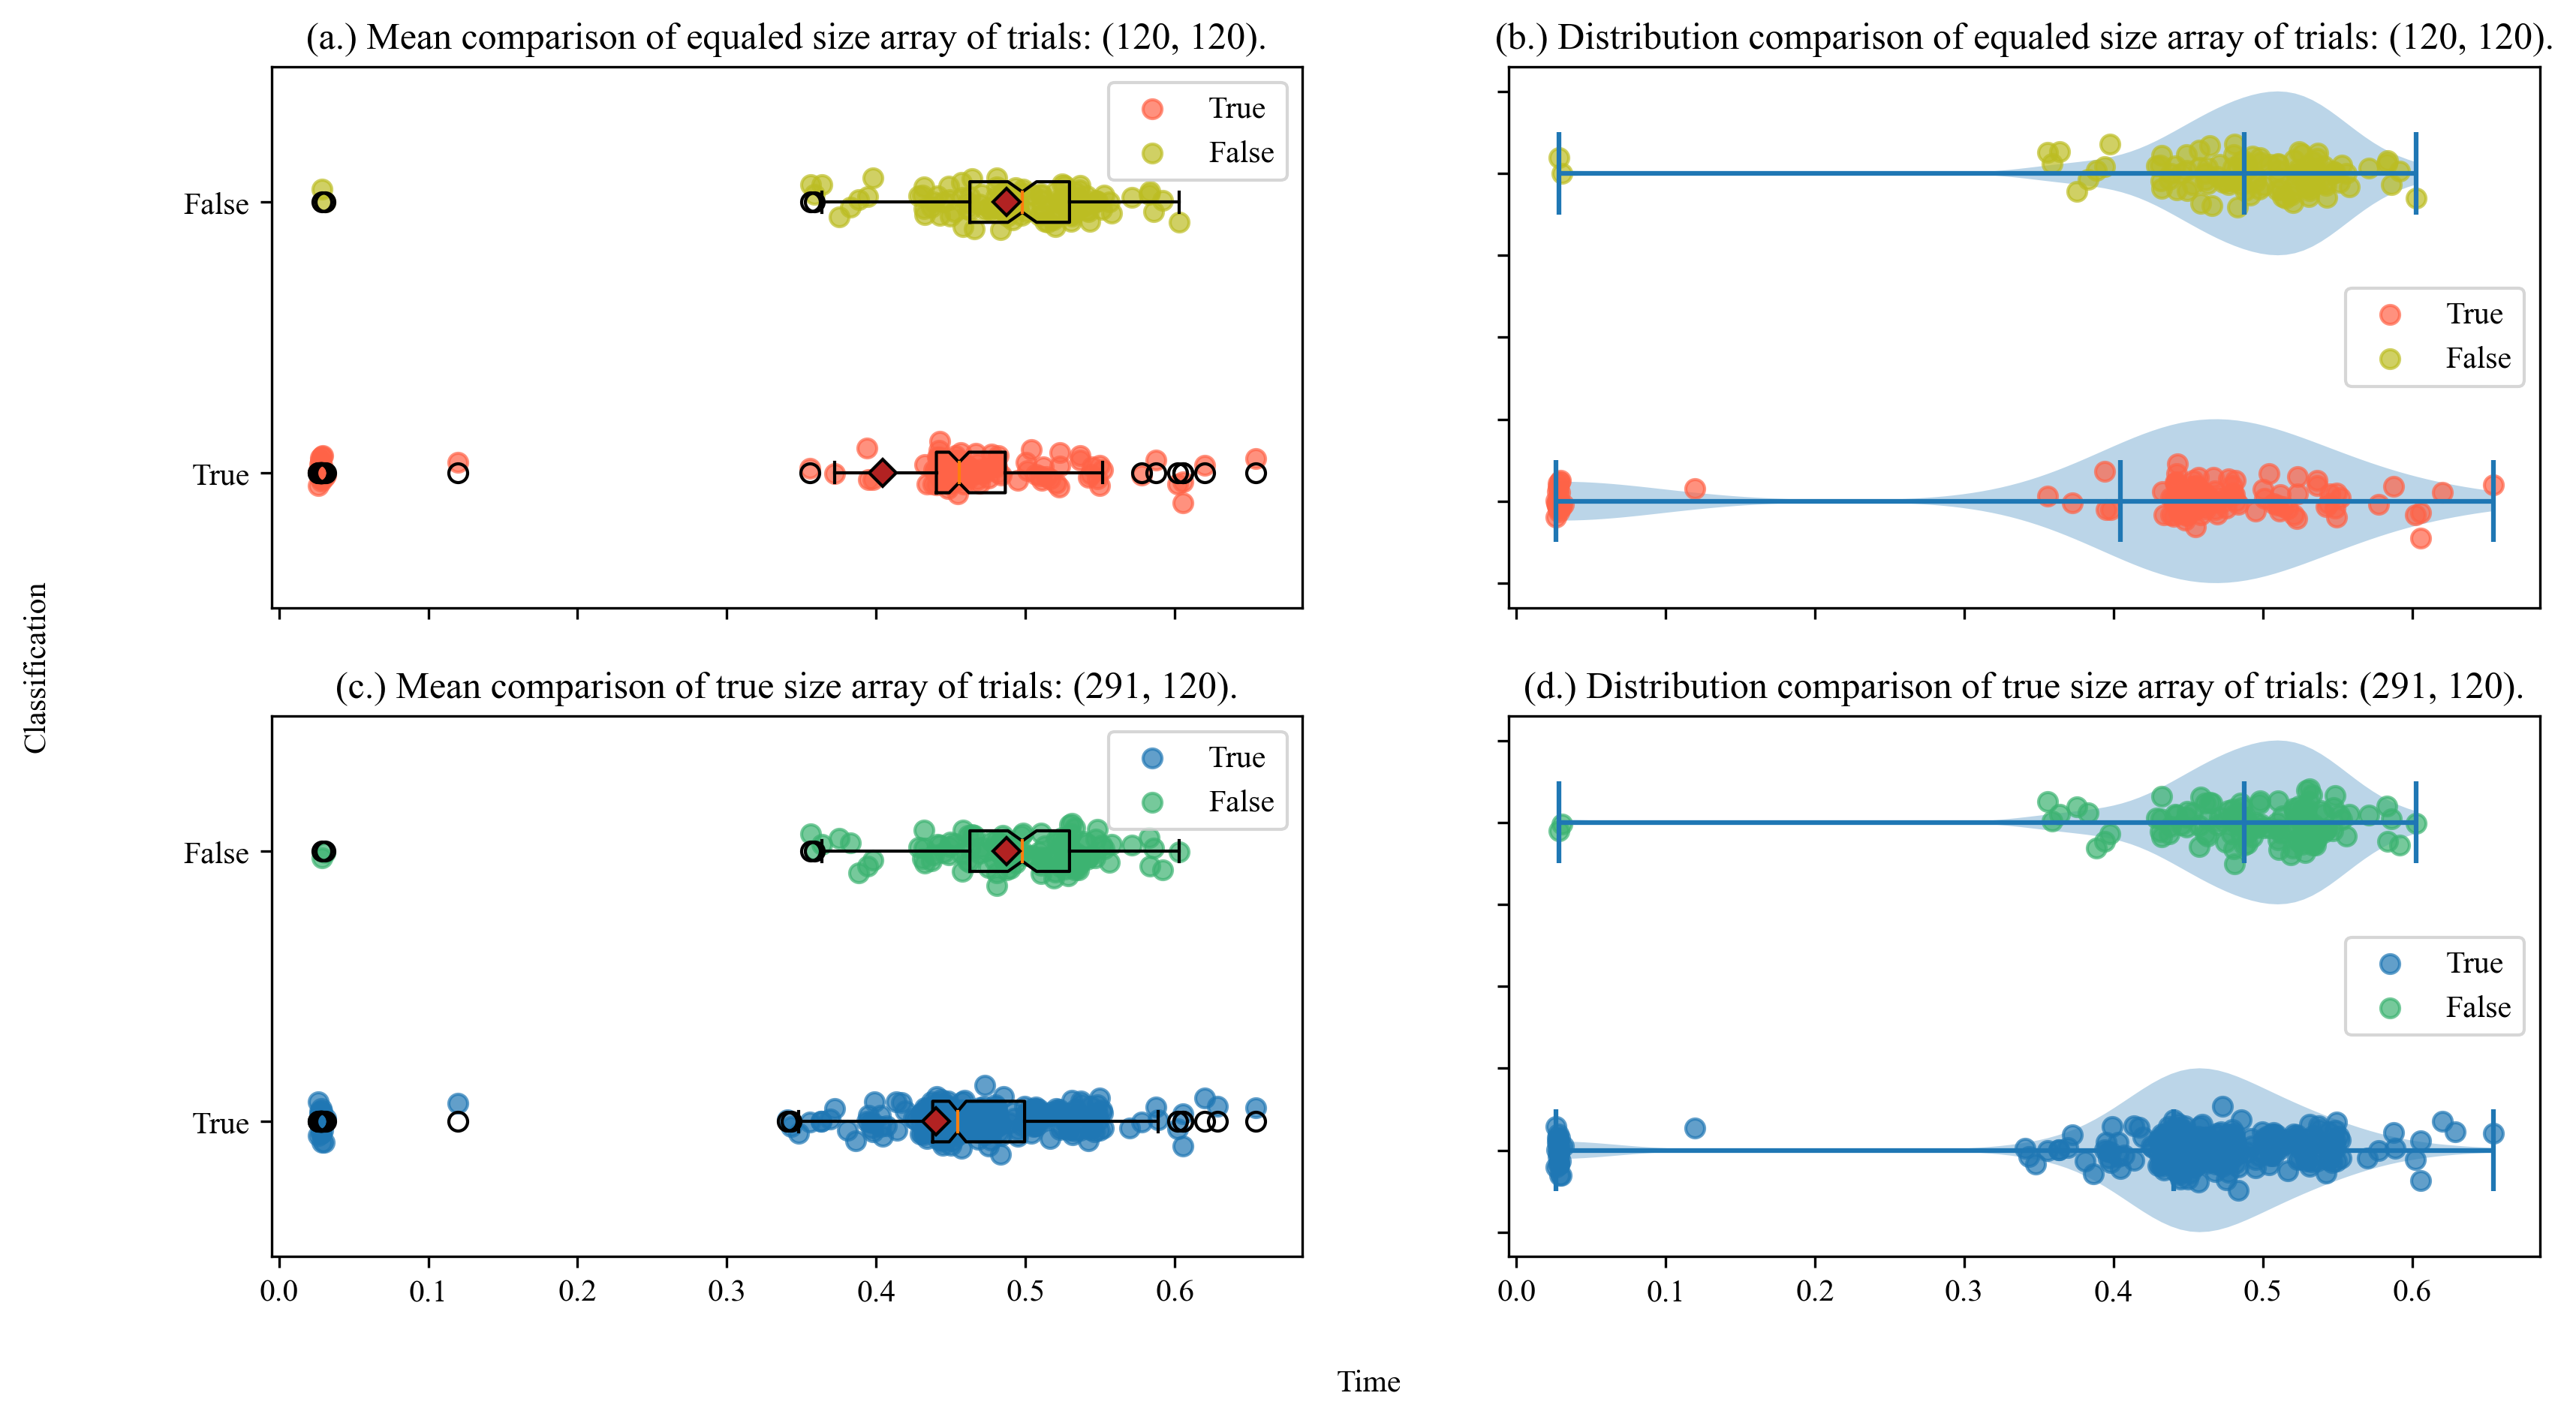
\includegraphics[width=\textwidth]{fig_2da.png}
	\caption{\doublespacing Comparison of average mean and distribution of time trials from 411 trials including random faces. (a.) and (b.) Presents the data of equal size ($N$) of array (\texttt{False}: 120 vs \texttt{True}: 120/291), and (c.) and (d.) Presents the data of the whole array (\texttt{False}: 120 vs \texttt{True}: 291), except for \texttt{NaN} data type (Not a Number from \texttt{pandas}), since $n > 0$\centering}. \label{fig:8}
\end{figure}

Concerning the speed and execution of the algorithm provided with the program, as exhibited by Figure \ref{fig:8}, averages on, $\mu_{\texttt{True}} = 0.440194808185567s \longrightarrow 0.44s \pm 0.05s$ for correct classification of faces, and $\mu_{\texttt{False}} = 0.4873850283166667s \longrightarrow 0.49s \pm 0.05s$ for wrong classification, on an \texttt{amd64} system with Linux kernel of \texttt{5.17.7-300.fc36.x86\_64} $\longrightarrow$ \texttt{5.17.7} inside virtual environment of Python 3.10.4, image container (Toolbox ), and \texttt{udev} rules of 10\% CPU utilization, and further specifications given by Listings 3.

\singlespacing
\begin{lstlisting}[caption={Specification of system from \texttt{lscpu} and \texttt{dmidecode}}]
$ lscpu
Architecture:            x86_64
	CPU op-mode(s):        32-bit, 64-bit
	Address sizes:         39 bits physical, 48 bits virtual
	Byte Order:            Little Endian
CPU(s):                  8
	On-line CPU(s) list:   0-7
Vendor ID:               GenuineIntel
	Model name:            Intel(R) Core(TM) i5-10210U CPU @ 1.60GHz
		CPU family:          6
		Model:               142
		Thread(s) per core:  2
		Core(s) per socket:  4
		Socket(s):           1
		Stepping:            12
		CPU(s) scaling MHz:  19%
		CPU max MHz:         4200.0000
		CPU min MHz:         400.0000
		BogoMIPS:            4199.88
		Flags:               fpu vme de pse tsc msr pae mce cx8 apic sep mtrr pge mc
		a cmov pat pse36 clflush dts acpi mmx fxsr sse sse2 ss 
		ht tm pbe syscall nx pdpe1gb rdtscp lm constant_tsc art
		arch_perfmon pebs bts rep_good nopl xtopology nonstop_
		tsc cpuid aperfmperf pni pclmulqdq dtes64 monitor ds_cp
		l vmx est tm2 ssse3 sdbg fma cx16 xtpr pdcm pcid sse4_1
		sse4_2 x2apic movbe popcnt tsc_deadline_timer aes xsav
		e avx f16c rdrand lahf_lm abm 3dnowprefetch cpuid_fault
		epb invpcid_single ssbd ibrs ibpb stibp ibrs_enhanced 
		tpr_shadow vnmi flexpriority ept vpid ept_ad fsgsbase t
		sc_adjust bmi1 avx2 smep bmi2 erms invpcid mpx rdseed a
		dx smap clflushopt intel_pt xsaveopt xsavec xgetbv1 xsa
		ves dtherm ida arat pln pts hwp hwp_act_window hwp_epp 
		md_clear flush_l1d arch_capabilities
Virtualization features: 
	Virtualization:        VT-x
Caches (sum of all):     
	L1d:                   128 KiB (4 instances)
	L1i:                   128 KiB (4 instances)
	L2:                    1 MiB (4 instances)
	L3:                    6 MiB (1 instance)
NUMA:                    
	NUMA node(s):          1
	NUMA node0 CPU(s):     0-7
Vulnerabilities:         
	Itlb multihit:         KVM: Mitigation: VMX disabled
	L1tf:                  Not affected
	Mds:                   Not affected
	Meltdown:              Not affected
	Spec store bypass:     Mitigation; Speculative Store Bypass disabled via prctl
	Spectre v1:            Mitigation; usercopy/swapgs barriers and __user pointer
	sanitization
	Spectre v2:            Mitigation; Enhanced IBRS, IBPB conditional, RSB fillin
	g
	Srbds:                 Mitigation; TSX disabled
	Tsx async abort:       Not affected

$ dmidecode
Handle 0x0004, DMI type 4, 48 bytes
Processor Information
	Socket Designation: U3E1
	Type: Central Processor
	Family: Core i5
	Manufacturer: Intel(R) Corporation
	ID: EC 06 08 00 FF FB EB BF
	Signature: Type 0, Family 6, Model 142, Stepping 12
	Flags:
		FPU (Floating-point unit on-chip)
		VME (Virtual mode extension)
		DE (Debugging extension)
		PSE (Page size extension)
		TSC (Time stamp counter)
		MSR (Model specific registers)
		PAE (Physical address extension)
		MCE (Machine check exception)
		CX8 (CMPXCHG8 instruction supported)
		APIC (On-chip APIC hardware supported)
		SEP (Fast system call)
		MTRR (Memory type range registers)
		PGE (Page global enable)
		MCA (Machine check architecture)
		CMOV (Conditional move instruction supported)
		PAT (Page attribute table)
		PSE-36 (36-bit page size extension)
		CLFSH (CLFLUSH instruction supported)
		DS (Debug store)
		ACPI (ACPI supported)
		MMX (MMX technology supported)
		FXSR (FXSAVE and FXSTOR instructions supported)
		SSE (Streaming SIMD extensions)
		SSE2 (Streaming SIMD extensions 2)
		SS (Self-snoop)
		HTT (Multi-threading)
		TM (Thermal monitor supported)
		PBE (Pending break enabled)
	Version: Intel(R) Core(TM) i5-10210U CPU @ 1.60GHz
	Voltage: 0.8 V
	External Clock: 100 MHz
	Max Speed: 8300 MHz
	Current Speed: 2574 MHz
	Status: Populated, Enabled
	Upgrade: Socket BGA1528
	L1 Cache Handle: 0x0005
	L2 Cache Handle: 0x0006
	L3 Cache Handle: 0x0007
	Serial Number: To Be Filled By O.E.M.
	Asset Tag: To Be Filled By O.E.M.
	Part Number: To Be Filled By O.E.M.
	Core Count: 4
	Core Enabled: 4
	Thread Count: 8
	Characteristics:
		64-bit capable
		Multi-Core
		Hardware Thread
		Execute Protection
		Enhanced Virtualization
		Power/Performance Control
		
Handle 0x0005, DMI type 7, 27 bytes
	Cache Information
	Socket Designation: L1 Cache
	Configuration: Enabled, Not Socketed, Level 1
	Operational Mode: Write Back
	Location: Internal
	Installed Size: 0 kB
	Maximum Size: 0 kB
	Supported SRAM Types:
	Synchronous
	Installed SRAM Type: Synchronous
	Speed: Unknown
	Error Correction Type: Parity
	System Type: Unified
	Associativity: 8-way Set-associative

Handle 0x0006, DMI type 7, 27 bytes
	Cache Information
	Socket Designation: L2 Cache
	Configuration: Enabled, Not Socketed, Level 2
	Operational Mode: Write Back
	Location: Internal
	Installed Size: 0 kB
	Maximum Size: 0 kB
	Supported SRAM Types:
	Synchronous
	Installed SRAM Type: Synchronous
	Speed: Unknown
	Error Correction Type: Single-bit ECC
	System Type: Unified
	Associativity: 4-way Set-associative

Handle 0x0007, DMI type 7, 27 bytes
	Cache Information
	Socket Designation: L3 Cache
	Configuration: Enabled, Not Socketed, Level 3
	Operational Mode: Write Back
	Location: Internal
	Installed Size: 0 kB
	Maximum Size: 0 kB
	Supported SRAM Types:
	Synchronous
	Installed SRAM Type: Synchronous
	Speed: Unknown
	Error Correction Type: Multi-bit ECC
	System Type: Unified
	Associativity: 12-way Set-associative

Handle 0x0008, DMI type 10, 6 bytes
	On Board Device Information
	Type: Video
	Status: Enabled
	Description: Video Graphics Controller

Handle 0x000D, DMI type 16, 23 bytes
	Physical Memory Array
	Location: System Board Or Motherboard
	Use: System Memory
	Error Correction Type: None
	Maximum Capacity: 32 GB
	Error Information Handle: No Error
	Number Of Devices: 2

Handle 0x000E, DMI type 17, 40 bytes
	Memory Device
	Array Handle: 0x000D
	Error Information Handle: No Error
	Total Width: 64 bits
	Data Width: 64 bits
	Size: 8 GB
	Form Factor: SODIMM
	Set: None
	Locator: ChannelA-DIMM0
	Bank Locator: BANK 0
	Type: DDR4
	Type Detail: Synchronous
	Speed: 2667 MT/s
	Manufacturer: Transcend
	Serial Number: 00005907
	Asset Tag: 9876543210
	Part Number: JM2666HSG-8G        
	Rank: 1
	Configured Memory Speed: 2667 MT/s
	Minimum Voltage: 1.5 V
	Maximum Voltage: 1.5 V
	Configured Voltage: 1.2 V

Handle 0x000F, DMI type 17, 40 bytes
	Memory Device
	Array Handle: 0x000D
	Error Information Handle: No Error
	Total Width: 64 bits
	Data Width: 64 bits
	Size: 4 GB
	Form Factor: SODIMM
	Set: None
	Locator: ChannelB-DIMM0
	Bank Locator: BANK 2
	Type: DDR4
	Type Detail: Synchronous
	Speed: 3200 MT/s
	Manufacturer: Micron
	Serial Number: 00000000
	Asset Tag: 9876543210
	Part Number: 4ATF51264HZ-3G2J1   
	Rank: 1
	Configured Memory Speed: 2667 MT/s
	Minimum Voltage: 1.5 V
	Maximum Voltage: 1.5 V
	Configured Voltage: 1.2 V
	
Handle 0x0011, DMI type 20, 35 bytes
	Memory Device Mapped Address
	Starting Address: 0x00000000000
	Ending Address: 0x001FFFFFFFF
	Range Size: 8 GB
	Physical Device Handle: 0x000E
	Memory Array Mapped Address Handle: 0x0010
	Partition Row Position: Unknown
	Interleave Position: 1
	Interleaved Data Depth: 1

Handle 0x0012, DMI type 20, 35 bytes
	Memory Device Mapped Address
	Starting Address: 0x00000000000
	Ending Address: 0x000FFFFFFFF
	Range Size: 4 GB
	Physical Device Handle: 0x000F
	Memory Array Mapped Address Handle: 0x0010
	Partition Row Position: Unknown
	Interleave Position: 2
	Interleaved Data Depth: 1

\end{lstlisting}
\doublespacing

\begin{figure}[h!]
	\centering
	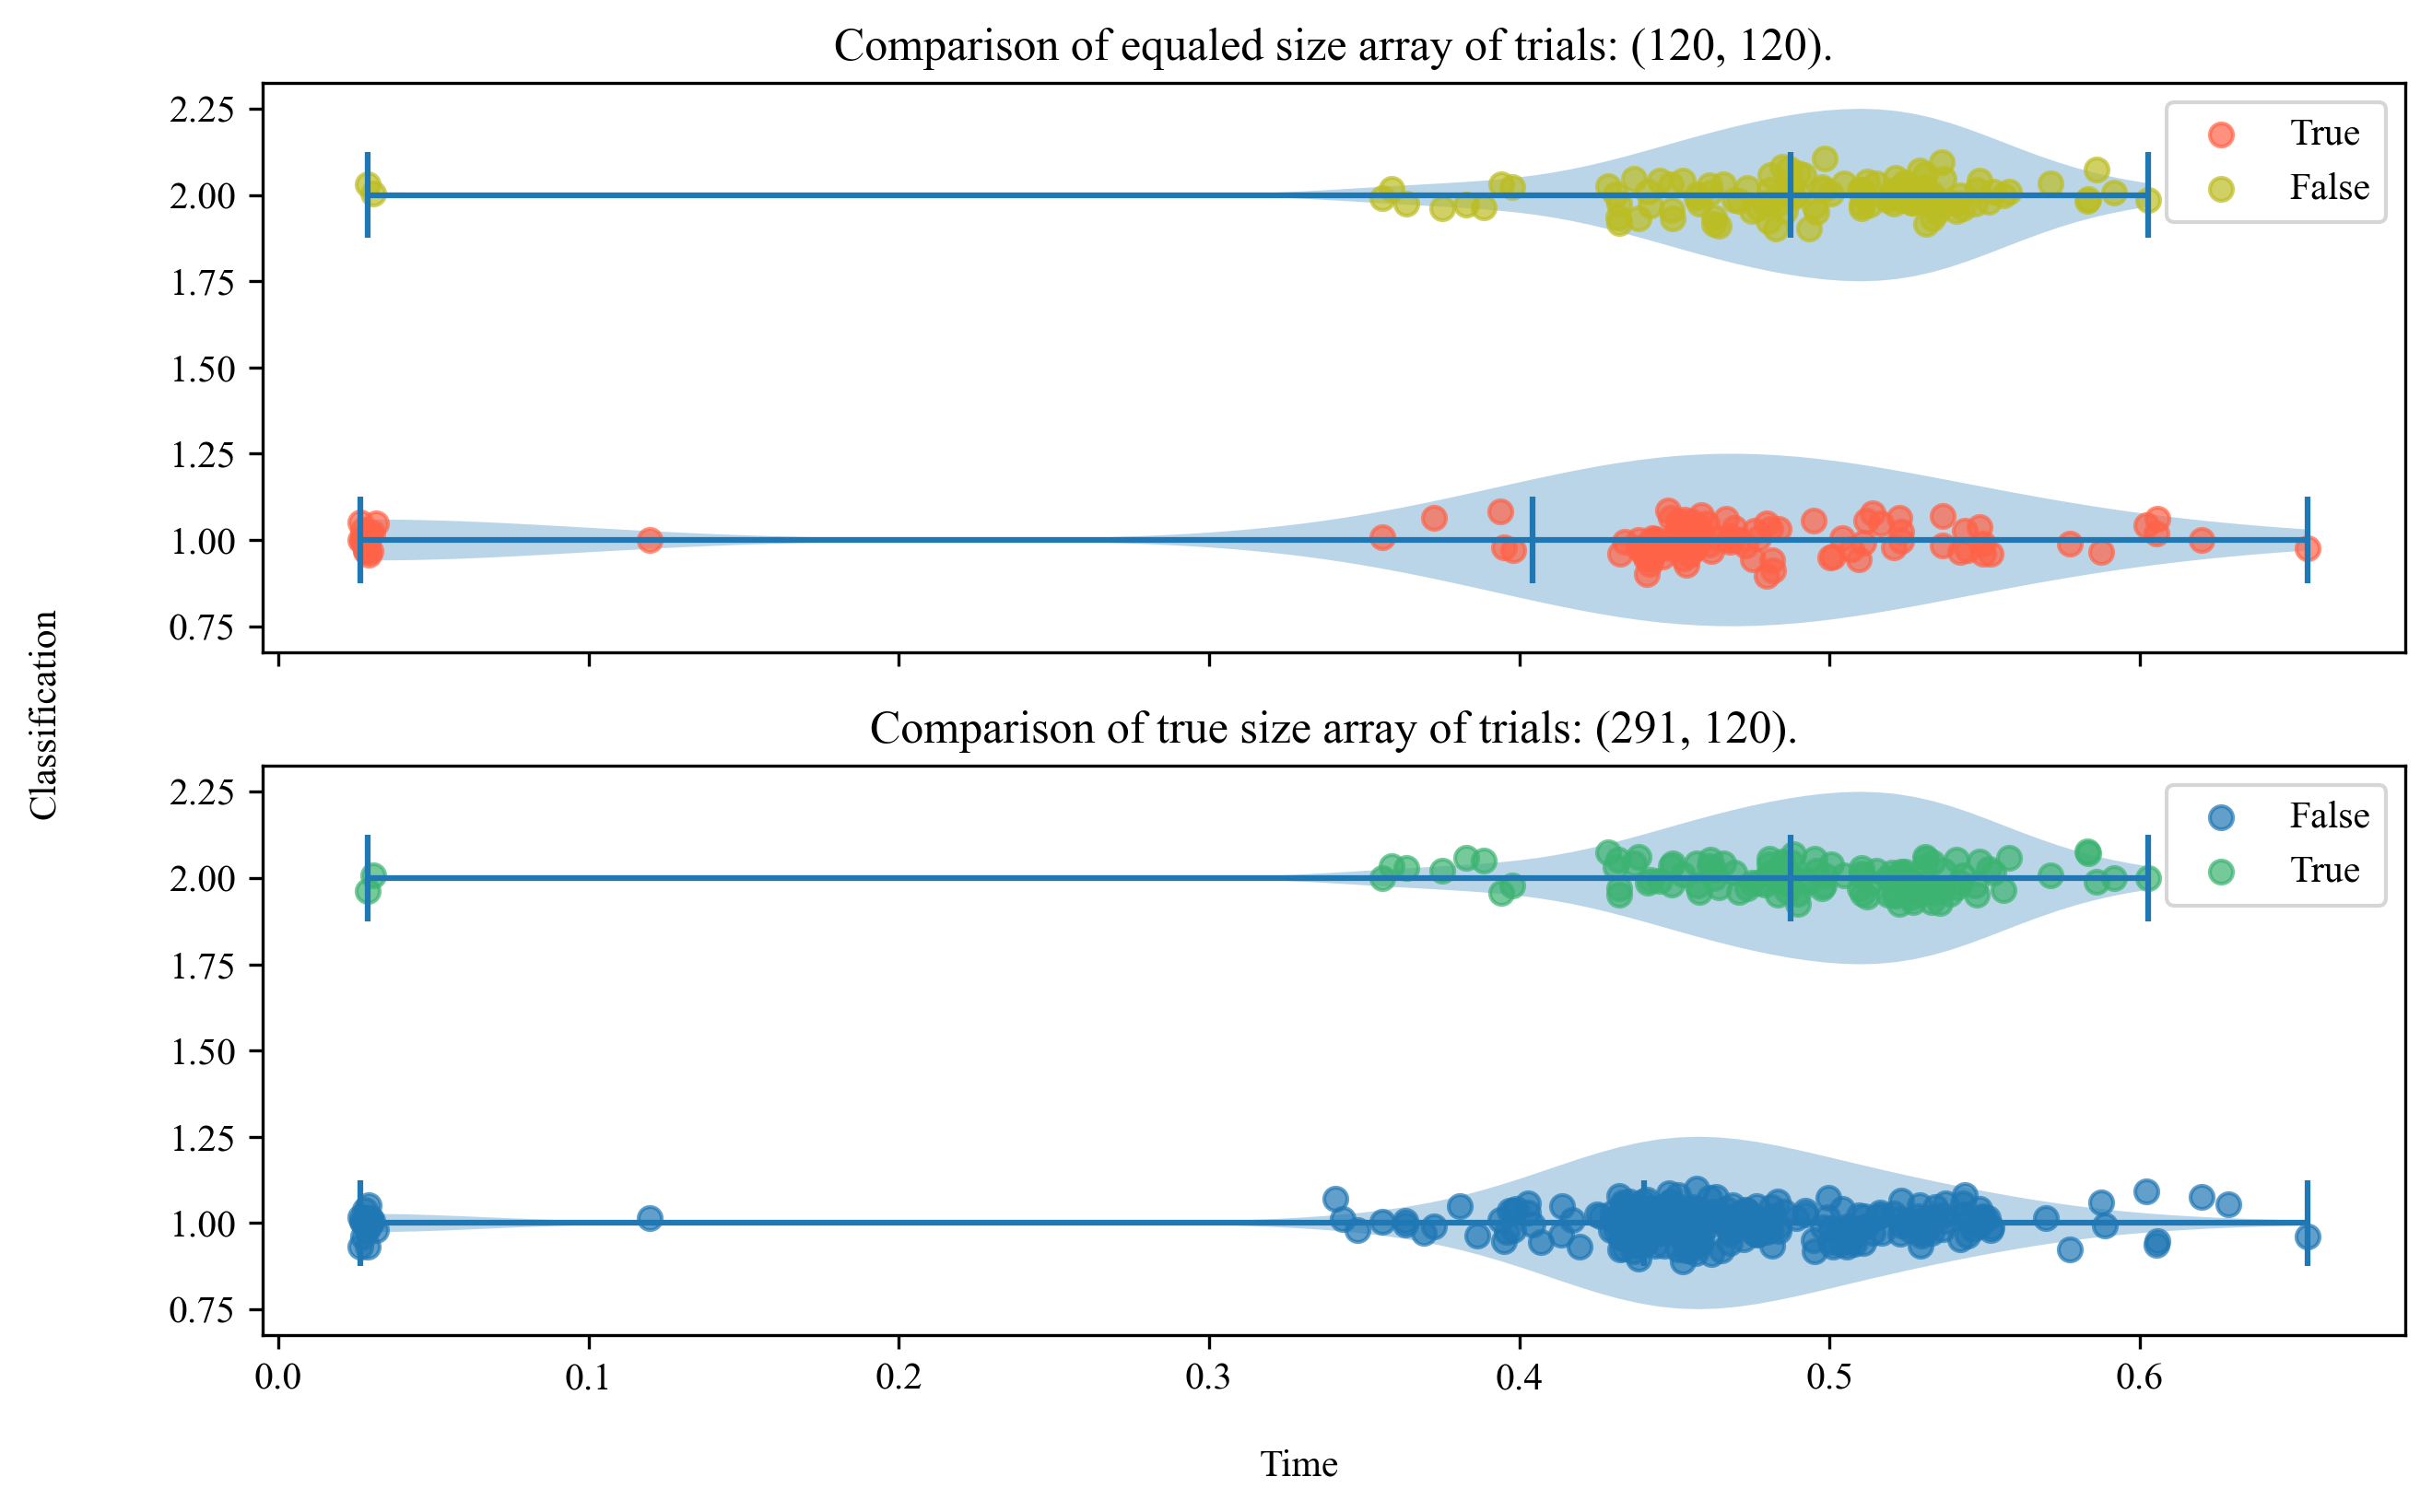
\includegraphics[width=\textwidth]{fig_1da.png}
	\caption{Time trials of face recognition-based attendance checking and security system.} \label{fig:9}
\end{figure}

The values collected, exhibited by Figure \ref{fig:9}, correspond to the specifications of the system presented by Listings above, since the processing of the data depends on the computation power of the system (Vopson, 2019; Vopson, 2022). And factoring the \texttt{udev} rules implemented in the system, that reduces the processing speed to at least $30\% \pm 20\%$, as well as the extra processes for data collection, this includes the call of \texttt{time.process\_command()} method to measure $\Delta t$ convert as \texttt{stdout} redirected (\texttt{>>}) to a file for data collection, where $t = 0$ was redeclared every loop as \texttt{decimal} datatype, the performance of the algorithm is above expectation.

\begin{figure}[h!]
	\centering
	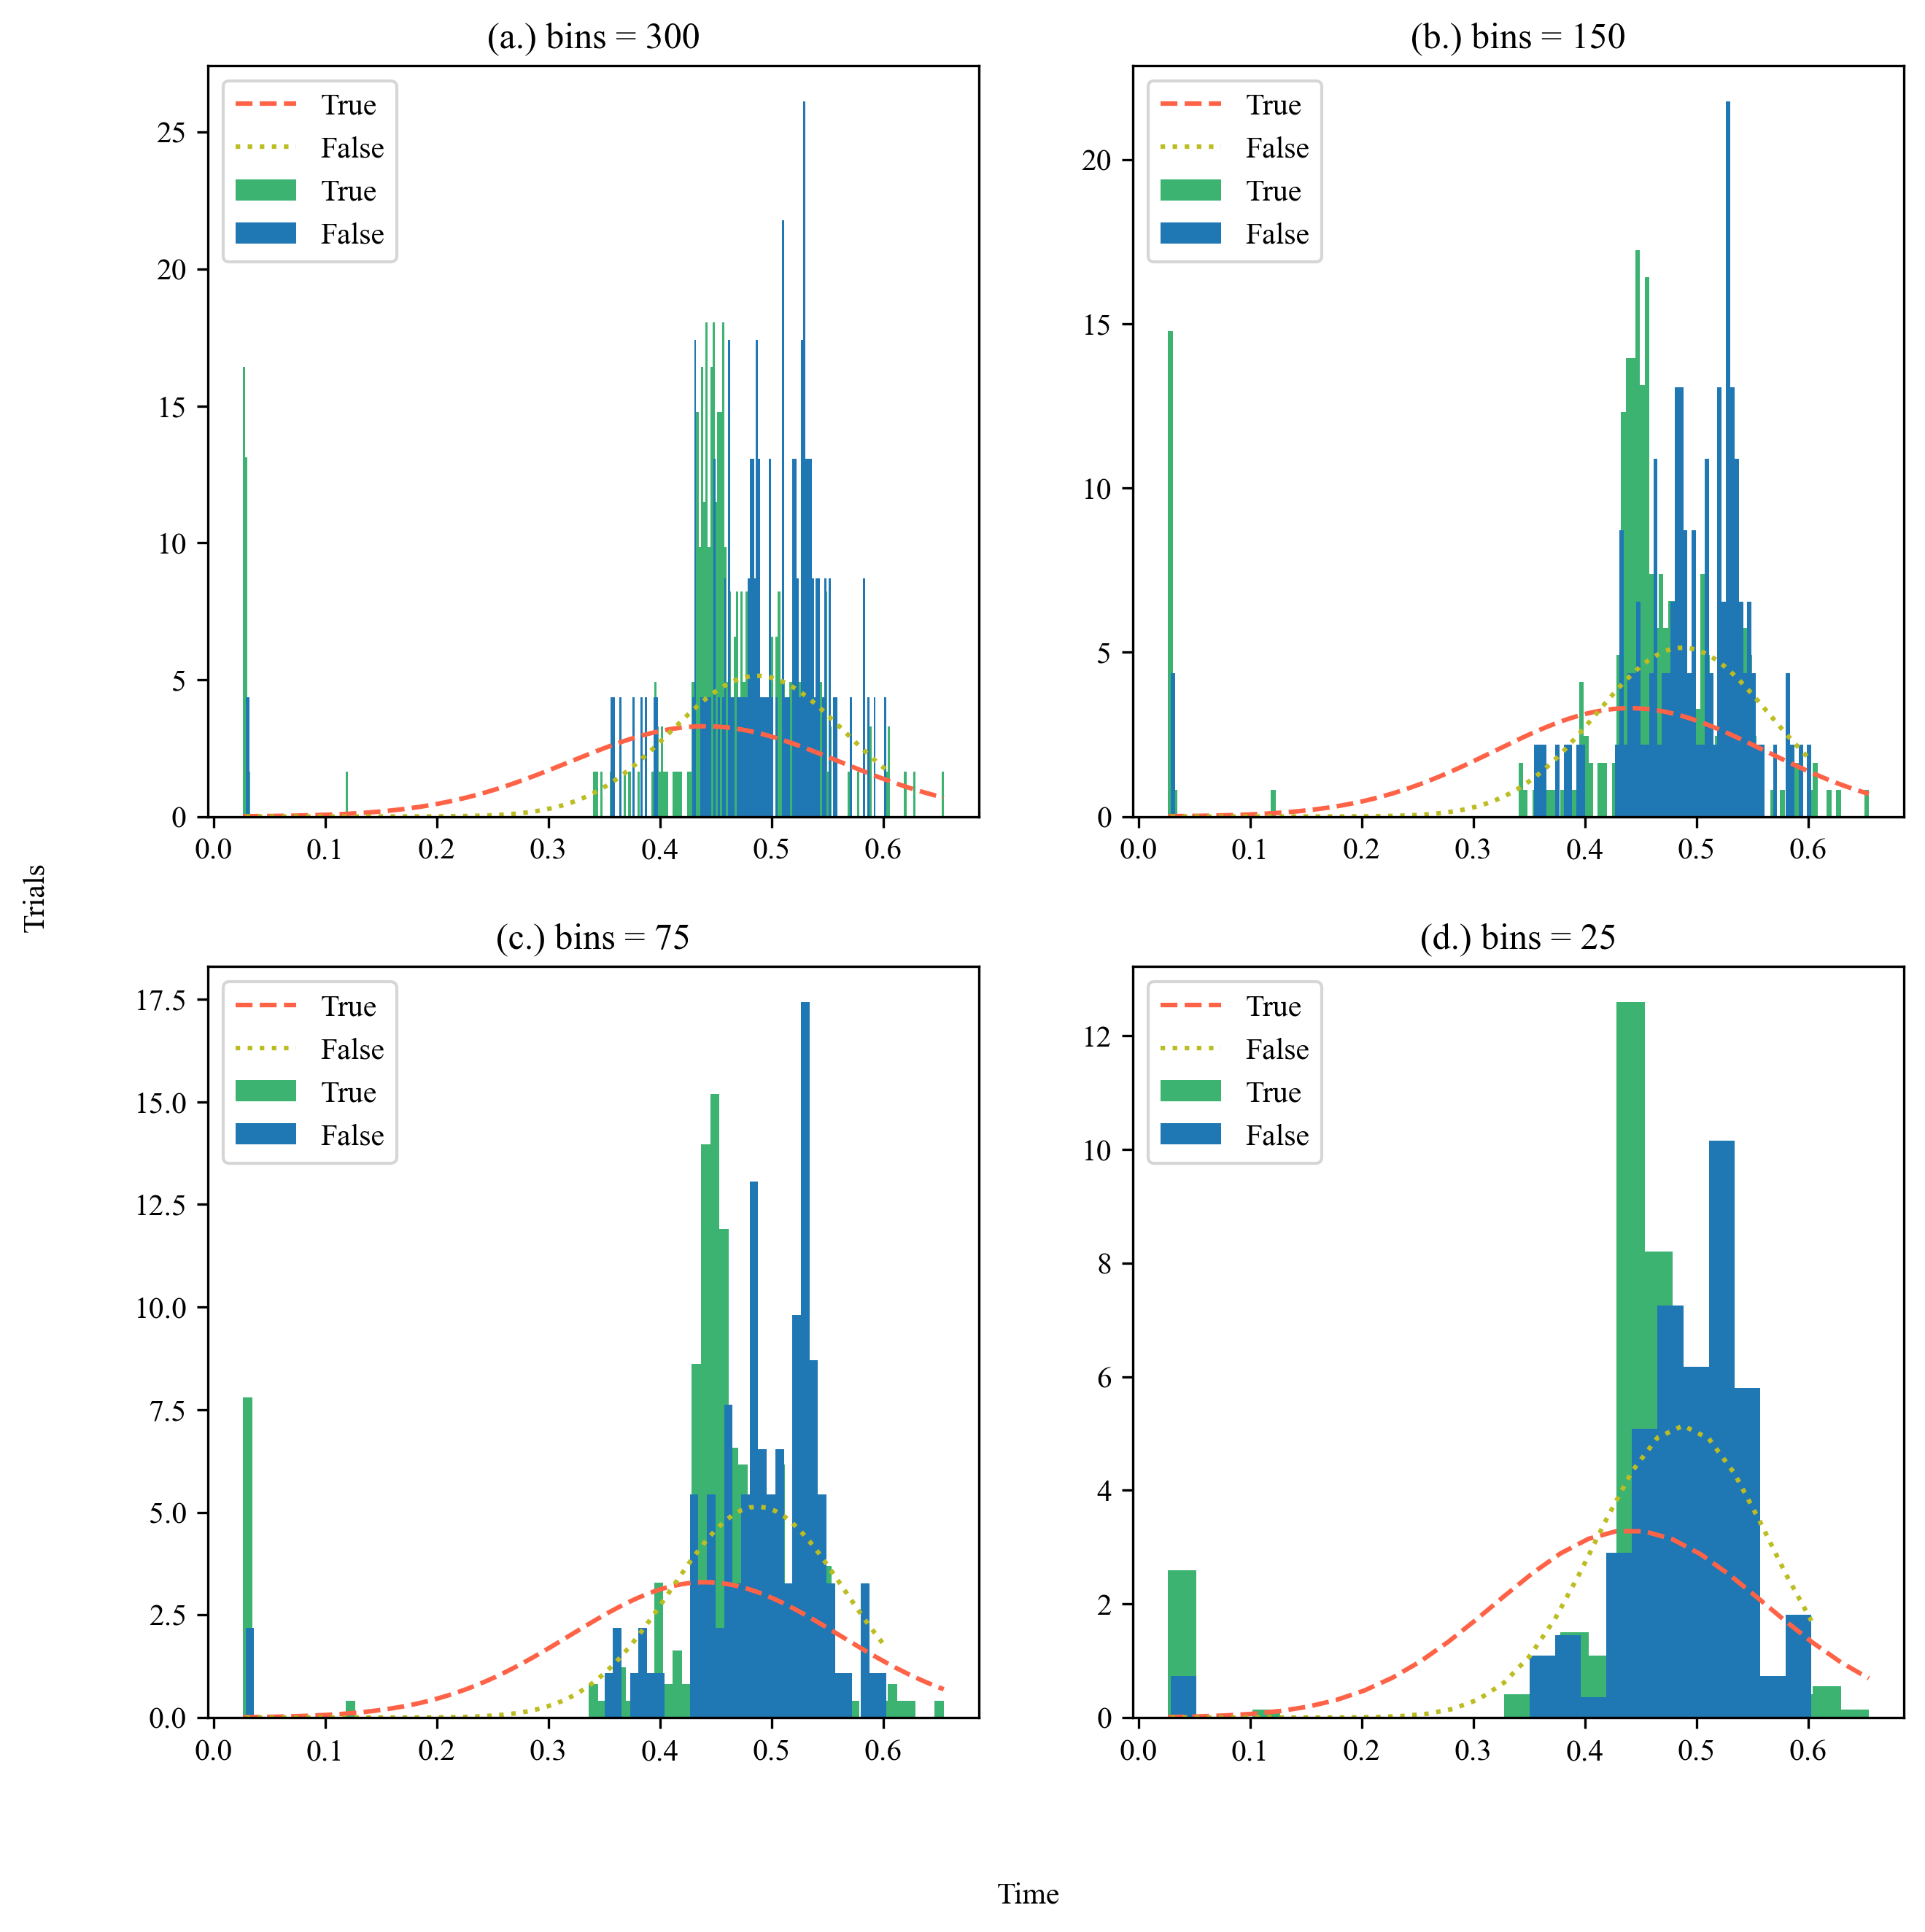
\includegraphics[width=\textwidth]{fig_3da.png}
	\caption{\doublespacing Time distributions of trials, starting from top-right, $bins = [300, 150, 75, 25]$.\centering}
\end{figure}

However, false classifications are also in significant amount which comprises $41.23\% \pm 1.000\%$ ($40\% \pm 1\%$) of the data, as presented by Figure 11. This is due to the early stages of the model, since the machine learning models are heavily dependent on the training data as well as new inputs (Jiang \etl, 2017, Shrestha \& Mahmood, 2019), it can be reasoned that the model did not managed to generate enough amount of weight per neurons and synapses (Shrestha \& Mahmood, 2019) to determine the best path in the layers for optimal output, since the input and data it requires for better classification and development of neural networks were not met.

And as opposed to common belief and perception, the efficiency and ability of model to correctly recognize faces is not time-dependent, since the model comparatively analyzes the encoding of faces, in reductive manner, thus allowing for fast and efficient recognition, in contrary to the depiction in science fictions, and other models, that a comparatively analyzes the input, in holistic manner.

It is also noted that algorithm creates two type of error, first is the Type I error, this occurs when the algorithm classified an unregistered face as face of a registered student, and the Type II error, if the algorithm classified a registered student as unknown. These type of errors were not explored, and was classified as \texttt{False}. This occurrence is caused by the confusion of facial features due to the almost similar samples, and due to the early stage of the model, as it did not have the sufficient amount of weight of neurons and synapses to correctly identify the facial features of each student, thus not giving the best output expected.

Nevertheless, a mean time of $\mu_{t} = 0.47s \pm 0.05s$ classification time on a computing power-limited system, the performance of the model can be considered above average. Moreover, the model can be transformed from its current state of unsupervised face recognition model, to a partially supervised model, whereas the model would prompt for confirmation upon confusion of inputs.

This allows the machine learning models of face recognition suitable for use in attendance checking and security systems application, considering that the model can be configured to improve in unsupervised manner in the later stages.

\subsubsection*{Regression Model of Prices of Arduino}

\begin{figure}[h!]
	\centering
	\includegraphics*[width=\textwidth]{fig_1r.png}
	\caption{\doublespacing Regression model of prices of Arduino from fluctuations of price from March 03, 2021 to May 17, 2022.\centering}	
\end{figure}

To model the cost efficiency of the systems, the researchers devised a linear regression model, with $\boldsymbol{x} :=$ demand, and $\boldsymbol{y}:= ln(price) e+2$ since price and demand has a perfect correlation, as shown by Pearson's Correlation Coefficient, $R = \frac{\sum (x-m_x)(y-m_y)}{\sqrt{\sum (x-m_x)^2 \sum (y - m_y)^2}}  = 1.0 \pm 0.1$ (performed by \texttt{scipy.stats.pearsonr(x, y)} provided by SciPy (\texttt{scipy})), shows a high precision and accuracy of the regression model, as presented by Figure 12.

\begin{figure}[h!]
	\centering
	\begin{subfigure}[b]{0.51\textwidth}
		\includegraphics*[width=\textwidth]{fig_3r.png}
		\subcaption{Combination of the regression model.}		
	\end{subfigure}
	\hfill
	\begin{subfigure}[b]{0.45\textwidth}
		\includegraphics*[width=\textwidth]{fig_2r.png}
		\subcaption{Breakdown of the regression model.}		
	\end{subfigure}
	\caption{\doublespacing Regression of prices in timeframes of: 12 months, 36 months, and 60 months, with mean of $\mu_{12 months} = 798.284359 \pm 5 PHP$, $\mu_{36 months} = 800.018379  \pm 5 PHP$, and $\mu_{60 months} = 801.532445  \pm 5 PHP$.\centering}
\end{figure}

Many individuals in the society are tend to think that cutting edge technologies are of high prices, rather unaffordable, and expensive to maintain, that can be explained by the socio-cultural background of an individual determined by social-learning interactions.

The models of basic perception of people towards specific matter depends on the social stereotype (Judd \& Park, 1993), which can be inaccurate and flawed (val Tilburg, Igou \&, Panjwani, 2022), but still contributes significantly to culture of an individual that plays a crucial role in the fast judgment, decision making, and perception towards specific matter (val Tilburg, Igou \&, Panjwani, 2022; DiMaggio, 1997). Moreover, the perception towards subject matter varies significantly from one person to another regardless of being with the same stereotype, since different individuals process and understand culture differently via different social-learning interactions, thus creating a difference before passing the learned information from one another, as only the individual can only be the source of cultural data (Handwerker, 2001).

Hence the perception of individuals in the society towards the expense of modern technology can be attributed to the socio-cultural background. In contrary to the commonly held belief by the society,  regression models of Arduino, suggests that RFID and Arduino-based systems are significantly more cost efficient than traditional methods that is in current use. Moreover, the model predicts that in the time frame of 60 months, the price of Arduino boards would decrease significantly, specifically decrease by $\mu_{decrease_{12 months}} = 20.74\% \pm 0.25\%$, $\mu_{decrease_{36 months}} = 20.84\% \pm 0.25\%$ and $\mu_{decrease_{60 months}} = 20.82\% \pm 0.25\%$, as depicted by Figure 13.

Since Arduino systems can last for long term use, with an estimated of $3 < time (years) < 10$, an 800 PHP RFID and Arduino-based lock access system is therefore more cost efficient than a 500 PHP/year\footnote{Assuming that a branded items were used.} lock maintenance and replacement of parts to ensure robustness on traditional lock access systems.

Moreover, the cost can be further decreased by utilizing other less expensive Arduino-based systems, it compromises the functionality and increases the complexity of the system, however. Nevertheless, it would still provide the most basic necessity for the use case and retain the security and convenience of the other model.

\newpage
\section*{SUMMARY CONCLUSION AND RECOMMENDATION\centering}

\subsection*{Summary of Findings\centering}

To determine whether cutting edge technologies, specifically RFID and Arduino-based systems, and machine learning models of face recognition, can be utilized and implemented as lock access system, and attendance checking and security system, respectively, the researchers devised and tested the models experimentally.

\subsection*{Conclusions\centering}

Based on the results, it is concluded that:

\begin{enumerate}
	\item RFID and Arduino-based systems, despite of the drawbacks caused by dependencies and other features, are more functional and efficient with an unlock and lock time of $\mu_{t_{lock}} = 2.80s \pm 0.10s$ and $\mu_{t_{unlock}} = 6.60s \pm 0.10s$, than traditional lock access system, with an average lock and unlock time of $5s < \mu_t$
	
	\item Due to the hidden lock system and string checking algorithm of RFID and Arduino-based lock access system, common form of lock bypassing methods, as well as hacking vulnerabilities, are rendered useless, and decreased significantly, respectively, providing a more secure and robust lock access system.
	
	\item Regardless of the early stages of the machine learning models of face recognition, and without any applied patches, the face recognition-based attendance checking and security system, exhibits an above average performance of $\approx 59\% \pm 1.0\%$ correct classifications at a mean time of $\mu_{t} = 0.47s \pm 0.05s$, in a limited power of machine at $30\% \pm 20\%$ core process.
		
	\item The linear regression models devised by the researchers suggests that RFID and Arduino based systems are significantly more cost efficient than traditional methods, and predicted that would be more cost efficient of at least $20.74\% \pm 0.25\%$, $20.84\% \pm 0.25\%$, and $20.82\% \pm 0.25\%$, in the following 12 months, 36 months, and 60 months, respectively.
	
\end{enumerate}

\subsection*{Recommendations\centering}

Based on the conclusions, these are recommended for further improvements:

\begin{enumerate}
	\item Improve the other parts of the lock access system, specifically:
	\begin{enumerate}
		\item LCD, by decrease the latency;
		\item utilize a high speed servo motor to decrease the unlock and lock time;
		\item avoid the use of external dependencies to increase speed of the algorithm;
		\item improve the module utilized for the hardware communication of the algorithm;
	\end{enumerate}
	\item Patch the algorithm to further decrease the classification time;
	\item Configure the machine learning models of face recognition to allow unsupervised learning from input;
	\item Transition the face recognition algorithm in partial supervision, to decrease the error rate;
	\item Further optimize the code base of the attendance checking and security system;
	\item Utilize other machine learning face recognition models;
	\item Further train the machine learning face recognition models;
	\item Evaluate the performance of other Arduino boards for use in lock access systems;
	\item Assess the perception of people towards the use of RFID technology and Arduino boards as lock access system, and machine learning models of face recognition as attendance checking and security system, in terms of:
	\begin{enumerate}
		\item convenience;
		\item sense of security;
		\item and sense of privacy;
	\end{enumerate}
	\item Compare the devised models with other commercially available models of RFID and Arduino-based lock access system, and face recognition-based attendance and security systems.
\end{enumerate}

\end{document}